\section{High Spatial Autocorrelation Results}
The methods will be compared on target fields generated with an autocorrelation factor, $\sigma_{field}$, equal to the field width.

\begin{figure}[htb!]
    \centering
    \begin{subfigure}[t]{0.25\textwidth}
        \centering
        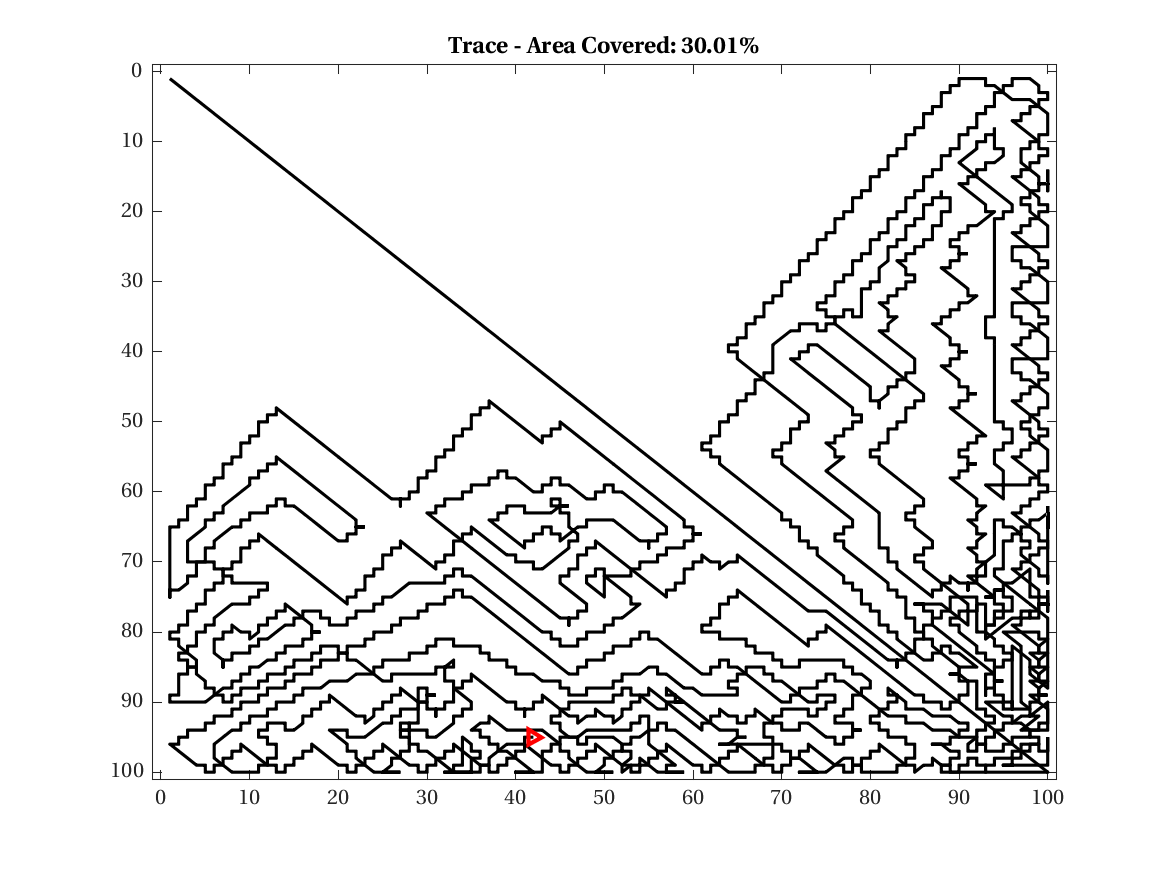
\includegraphics[width=\linewidth]{figures/path_greedy_30p_100x100_sf_100_seed_1.png}
        \captionsetup{skip=0.20\baselineskip,size=footnotesize}
        \caption{Greedy NBV}
    \end{subfigure}%
    \begin{subfigure}[t]{0.25\textwidth}
        \centering
        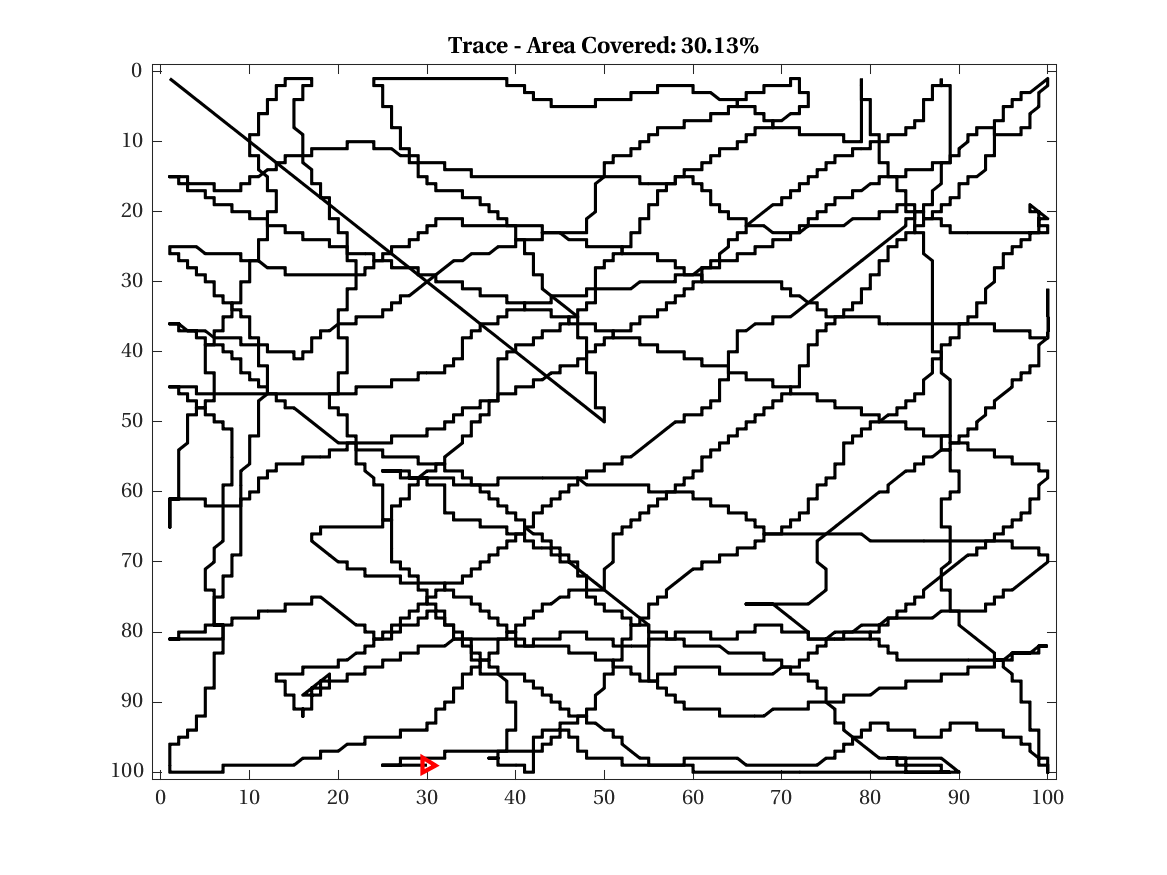
\includegraphics[width=\linewidth]{figures/path_mc_30p_100x100_sf_100_seed_1.png}
        \captionsetup{skip=0.20\baselineskip,size=footnotesize}
        \caption{MCPP}
    \end{subfigure}%
    \begin{subfigure}[t]{0.25\textwidth}
        \centering
        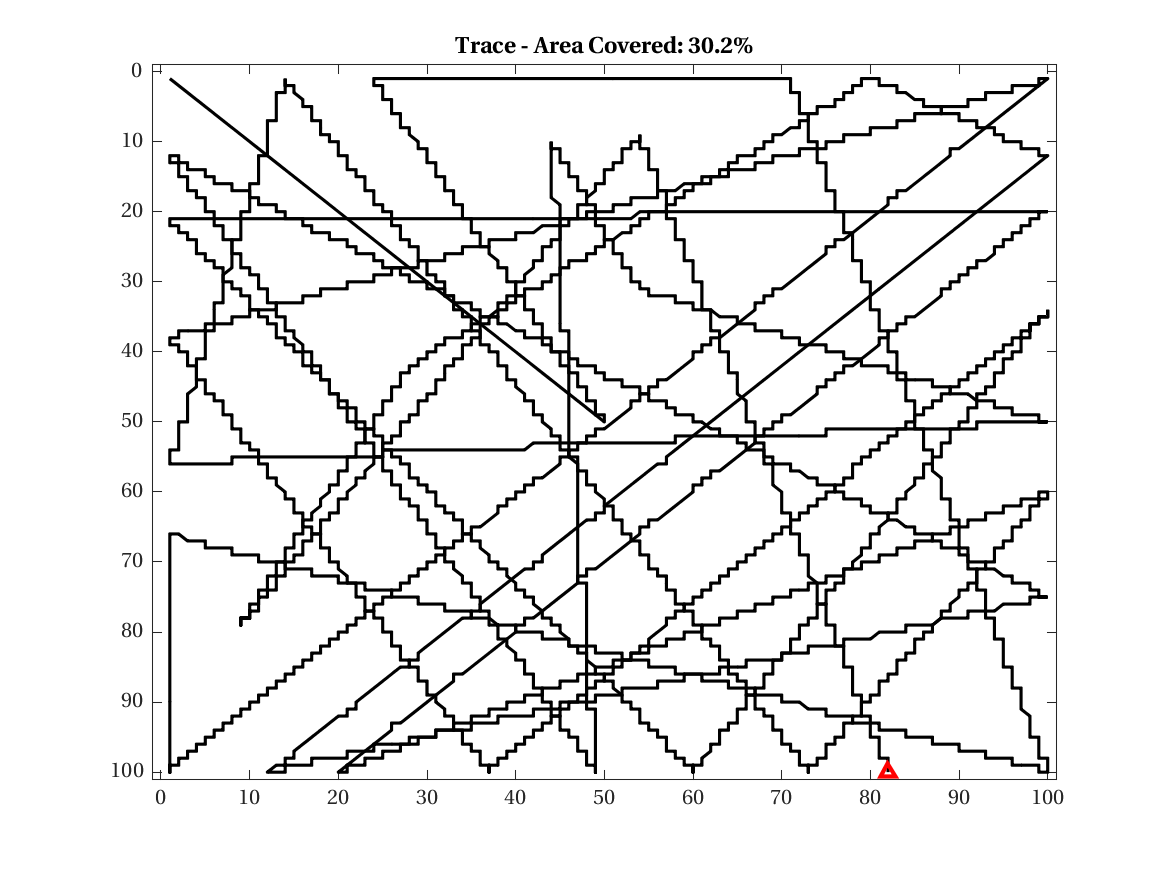
\includegraphics[width=\linewidth]{figures/path_nhv_30p_100x100_sf_100_seed_1.png}
        \captionsetup{skip=0.20\baselineskip,size=footnotesize}
        \caption{HV}
    \end{subfigure}%
    \begin{subfigure}[t]{0.25\textwidth}
        \centering
        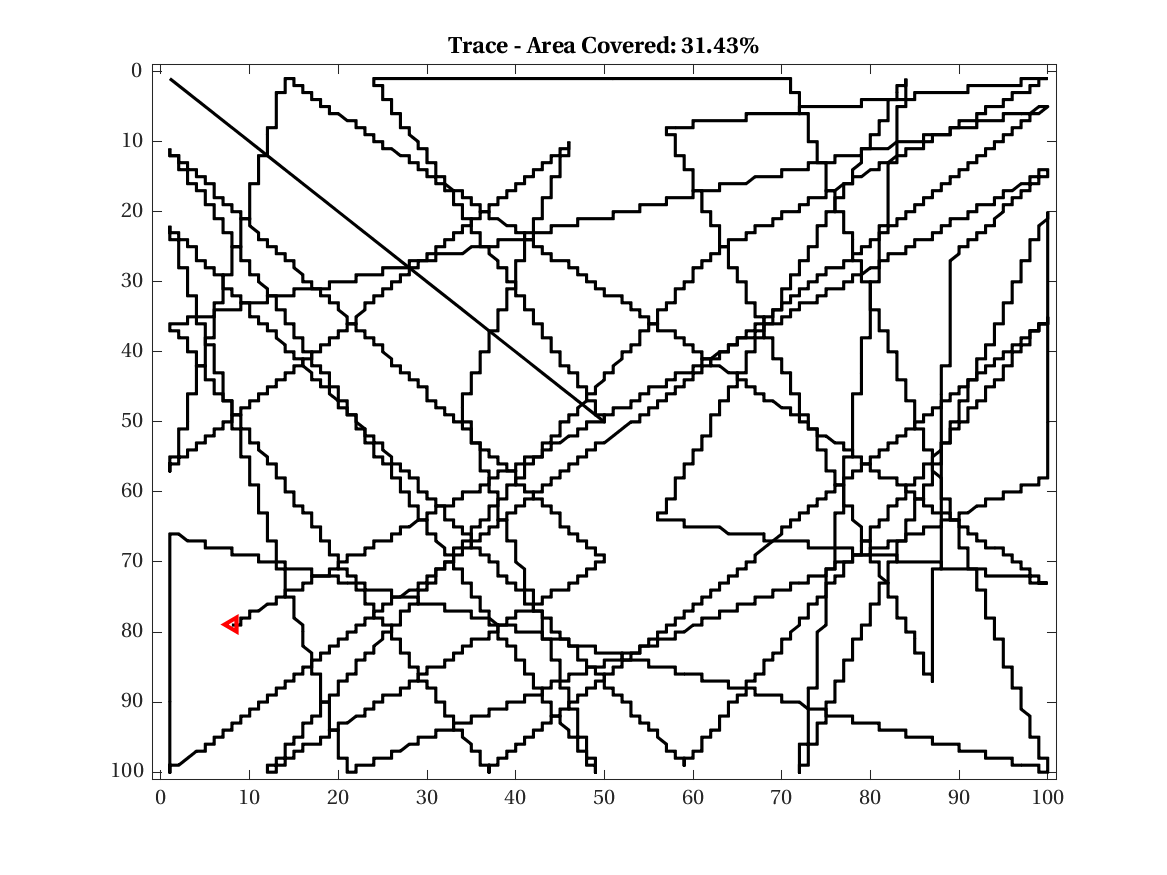
\includegraphics[width=\linewidth]{figures/path_nnhv_30p_100x100_sf_100_seed_1.png}
        \captionsetup{skip=0.20\baselineskip,size=footnotesize}
        \caption{$N$-HV}
    \end{subfigure}%
    \\
    \begin{subfigure}[t]{0.25\textwidth}
        \centering
        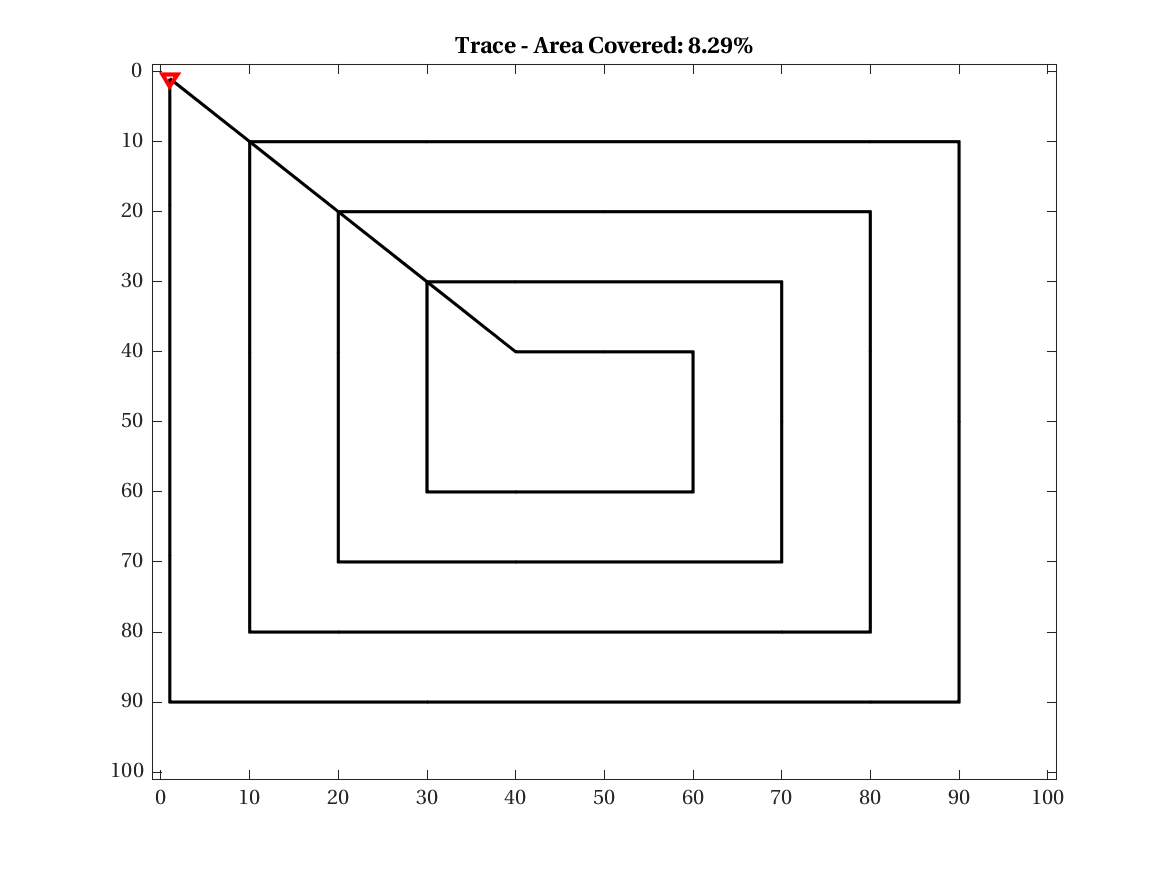
\includegraphics[width=\linewidth]{figures/path_zz_10p_100x100_sf_100_seed_1.png}
        \captionsetup{skip=0.20\baselineskip,size=footnotesize}
        \caption{$ZZ_{10}$}
    \end{subfigure}%
    \begin{subfigure}[t]{0.25\textwidth}
        \centering
        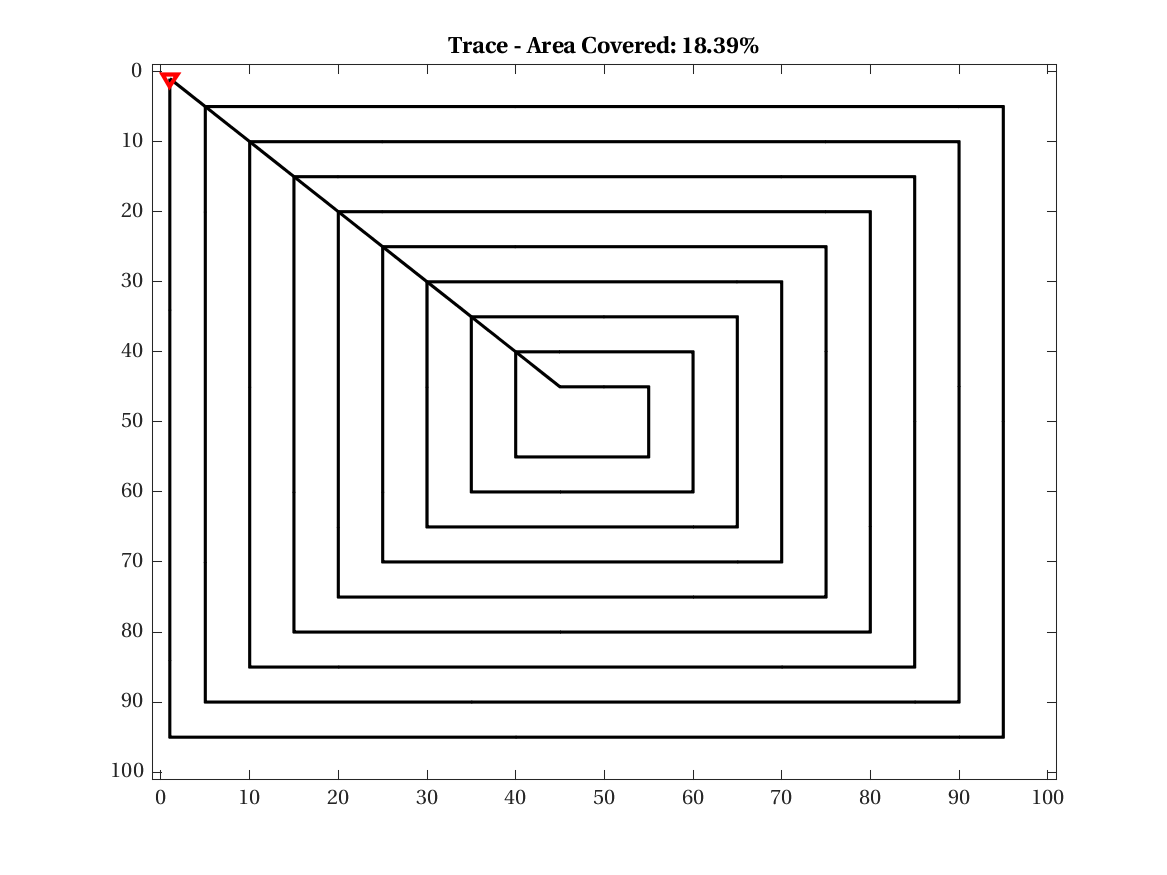
\includegraphics[width=\linewidth]{figures/path_zz_20p_100x100_sf_100_seed_1.png}
        \captionsetup{skip=0.20\baselineskip,size=footnotesize}
        \caption{$ZZ_{20}$}
    \end{subfigure}%
    \begin{subfigure}[t]{0.25\textwidth}
        \centering
        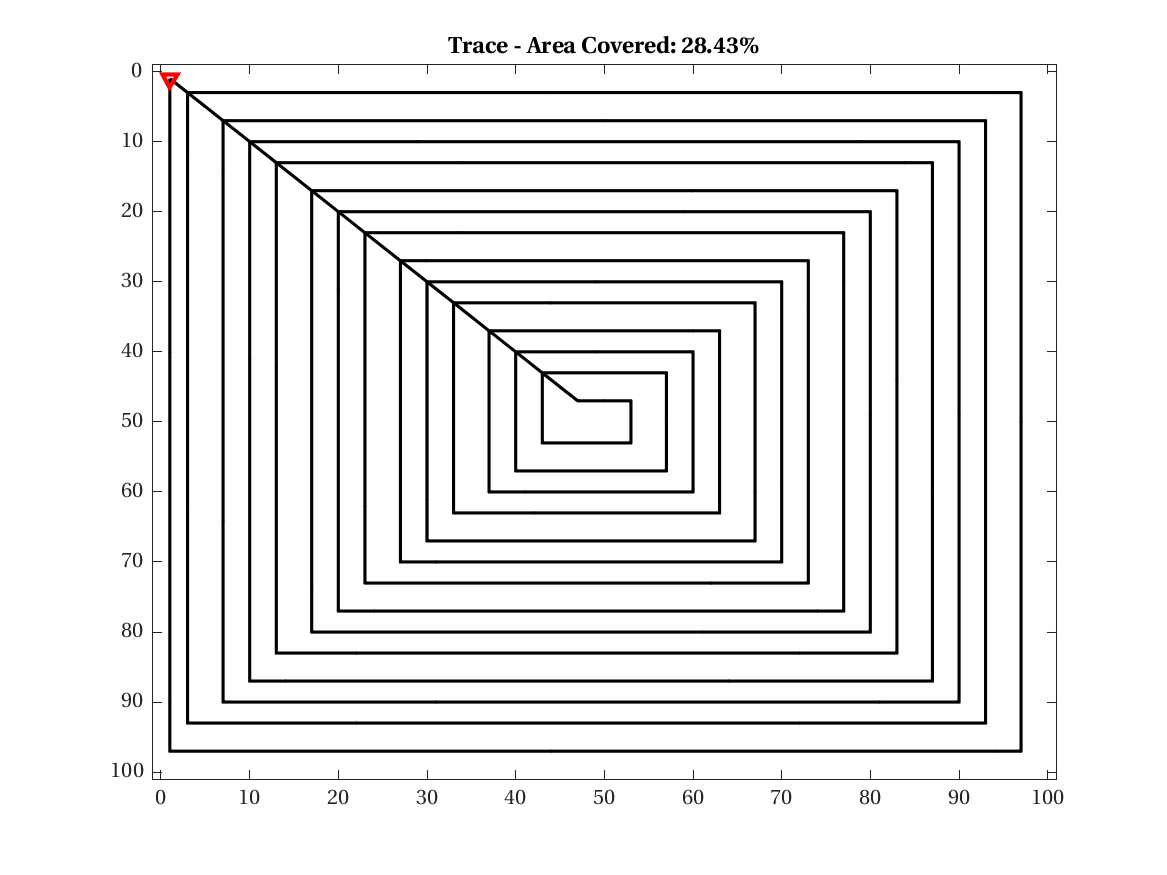
\includegraphics[width=\linewidth]{figures/path_zz_30p_100x100_sf_100_seed_1.png}
        \captionsetup{skip=0.20\baselineskip,size=footnotesize}
        \caption{$ZZ_{30}$}
    \end{subfigure}%
    \captionsetup{skip=0.20\baselineskip}
    \caption{Exploration of a field of size $100 \times 100$, $\sigma_{field} = 100$, random seed 1.}
    \label{fig:sf100}
\end{figure}

\begin{figure}[htb!]
    \centering
    \begin{subfigure}[t]{0.75\textwidth}
        \centering
        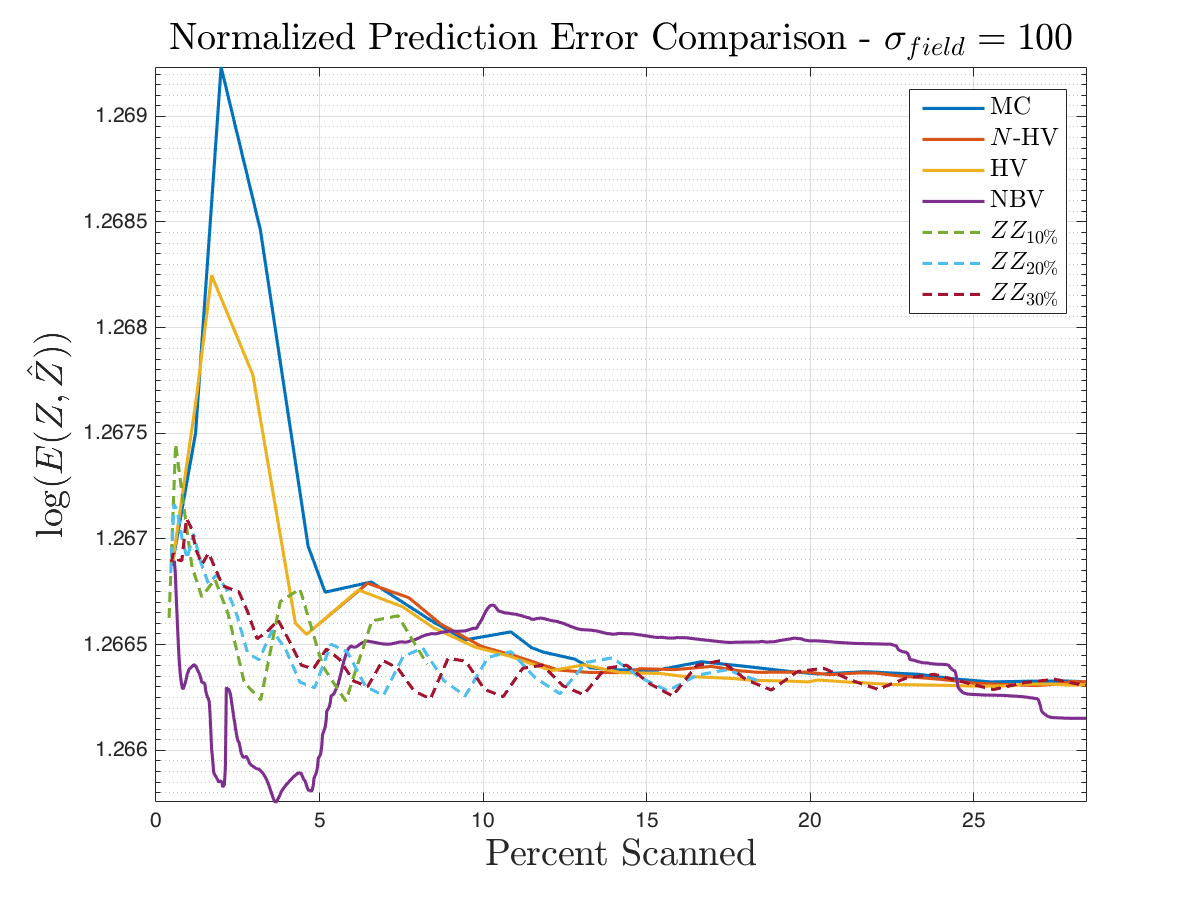
\includegraphics[width=\linewidth]{figures/normalized_errors_30p_100x100_sf_100_seed_1_app_10}
        \captionsetup{skip=0.20\baselineskip,size=footnotesize}
        \caption{Normalized prediction errors for each method.}
    \end{subfigure}%
    \\
    \begin{subfigure}[t]{0.75\textwidth}
        \centering
        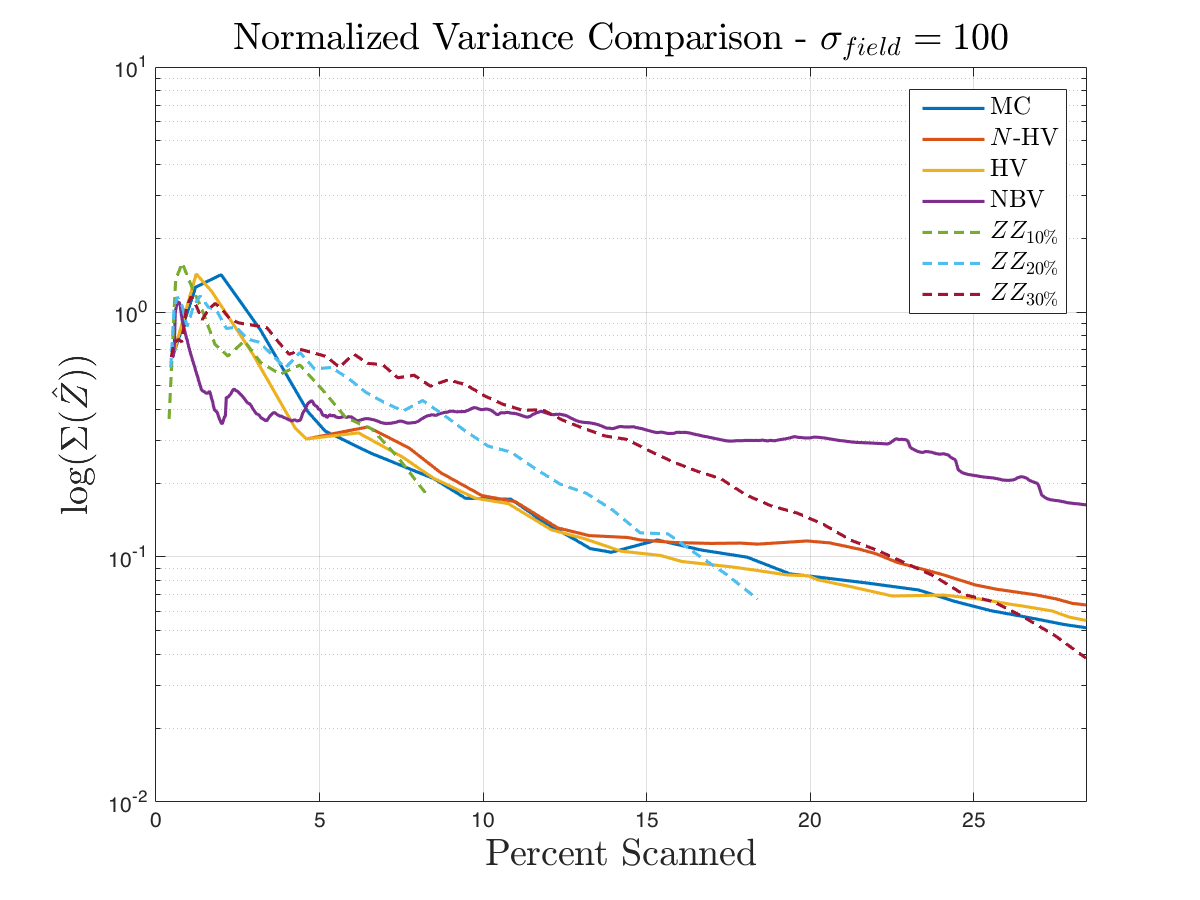
\includegraphics[width=\linewidth]{figures/normalized_variances_30p_100x100_sf_100_seed_1_app_10}
        \captionsetup{skip=0.20\baselineskip,size=footnotesize}
        \caption{Normalized prediction variances for each method.}
    \end{subfigure}%
    \captionsetup{skip=0.20\baselineskip}
    \caption{Prediction error and variances for an exploration of a field of size $100 \times 100$, $\sigma_{field} = 100$, random seed 1.}
    \label{fig:errvar100}
\end{figure}

\FloatBarrier
\clearpage\

\section{Half Width Spatial Autocorrelation Results}
The methods will be compared on target fields generated with an autocorrelation factor, $\sigma_{field}$, that is half of the field width.
\begin{figure}[htb!]
    \centering
    \begin{subfigure}[t]{0.25\textwidth}
        \centering
        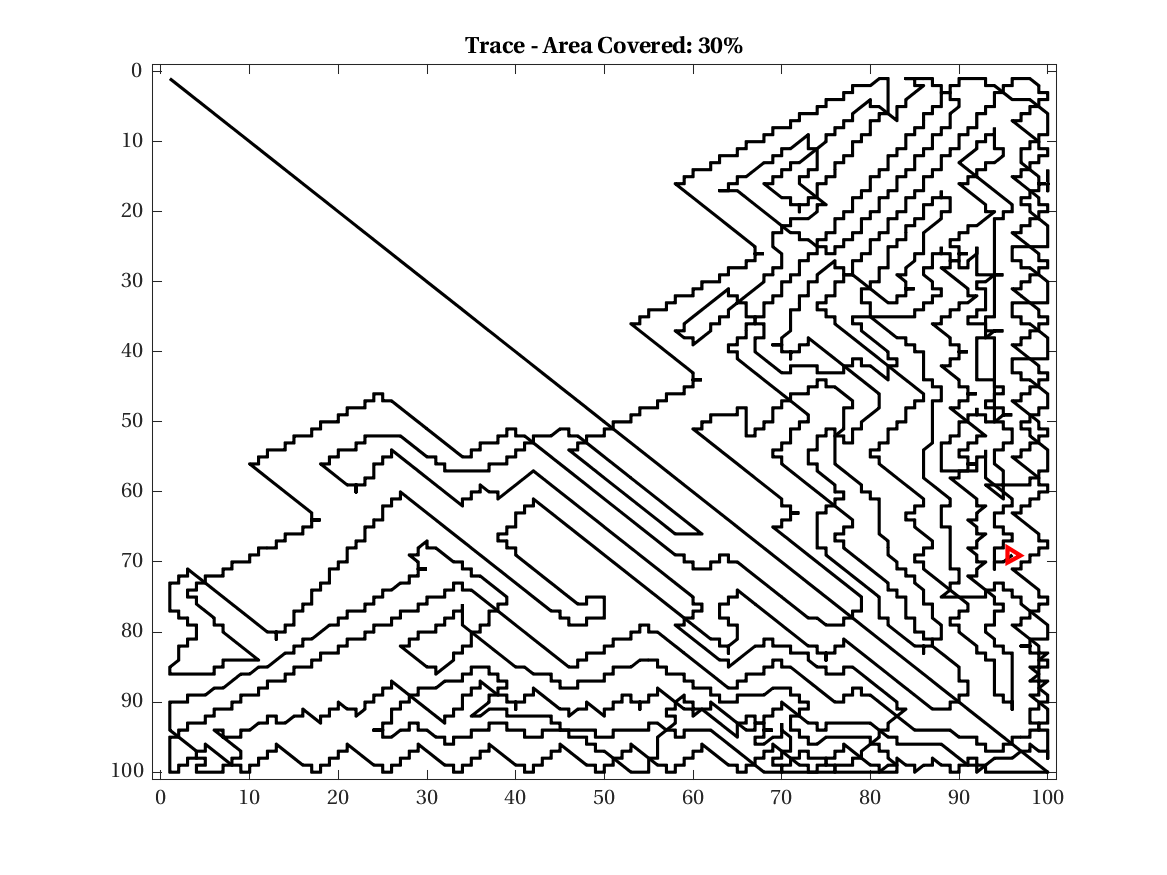
\includegraphics[width=\linewidth]{figures/path_greedy_30p_100x100_sf_50_seed_1.png}
        \captionsetup{skip=0.20\baselineskip,size=footnotesize}
        \caption{Greedy NBV}
    \end{subfigure}%
    \begin{subfigure}[t]{0.25\textwidth}
        \centering
        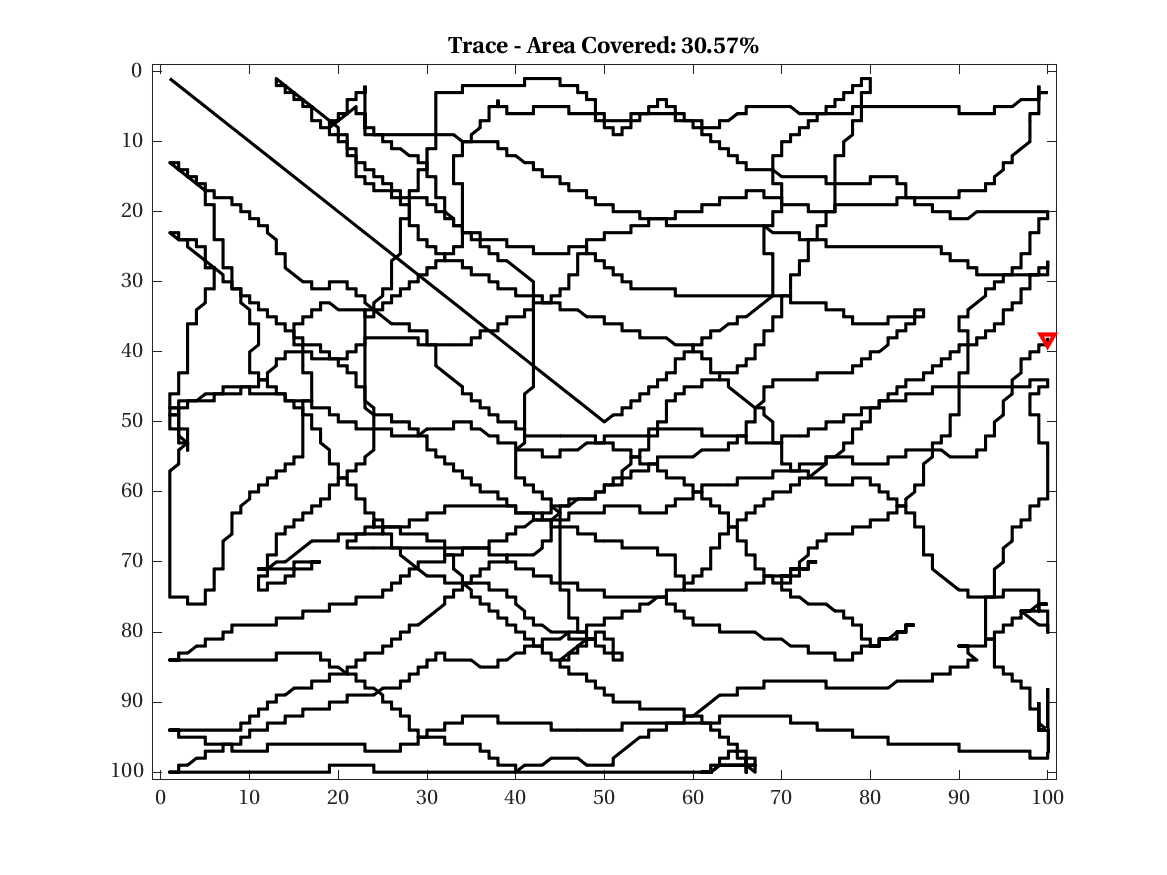
\includegraphics[width=\linewidth]{figures/path_mc_30p_100x100_sf_50_seed_1.png}
        \captionsetup{skip=0.20\baselineskip,size=footnotesize}
        \caption{MCPP}
    \end{subfigure}%
    \begin{subfigure}[t]{0.25\textwidth}
        \centering
        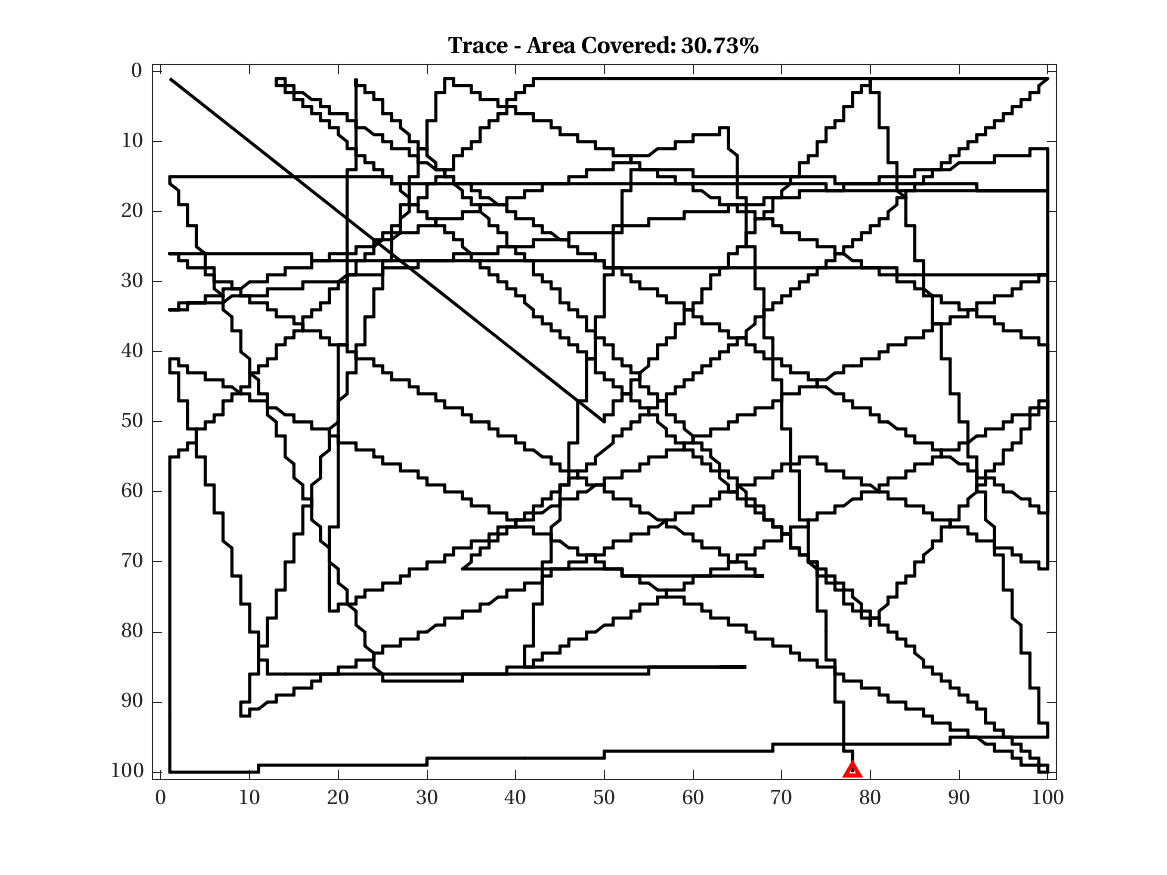
\includegraphics[width=\linewidth]{figures/path_nhv_30p_100x100_sf_50_seed_1.png}
        \captionsetup{skip=0.20\baselineskip,size=footnotesize}
        \caption{HV}
    \end{subfigure}%
    \begin{subfigure}[t]{0.25\textwidth}
        \centering
        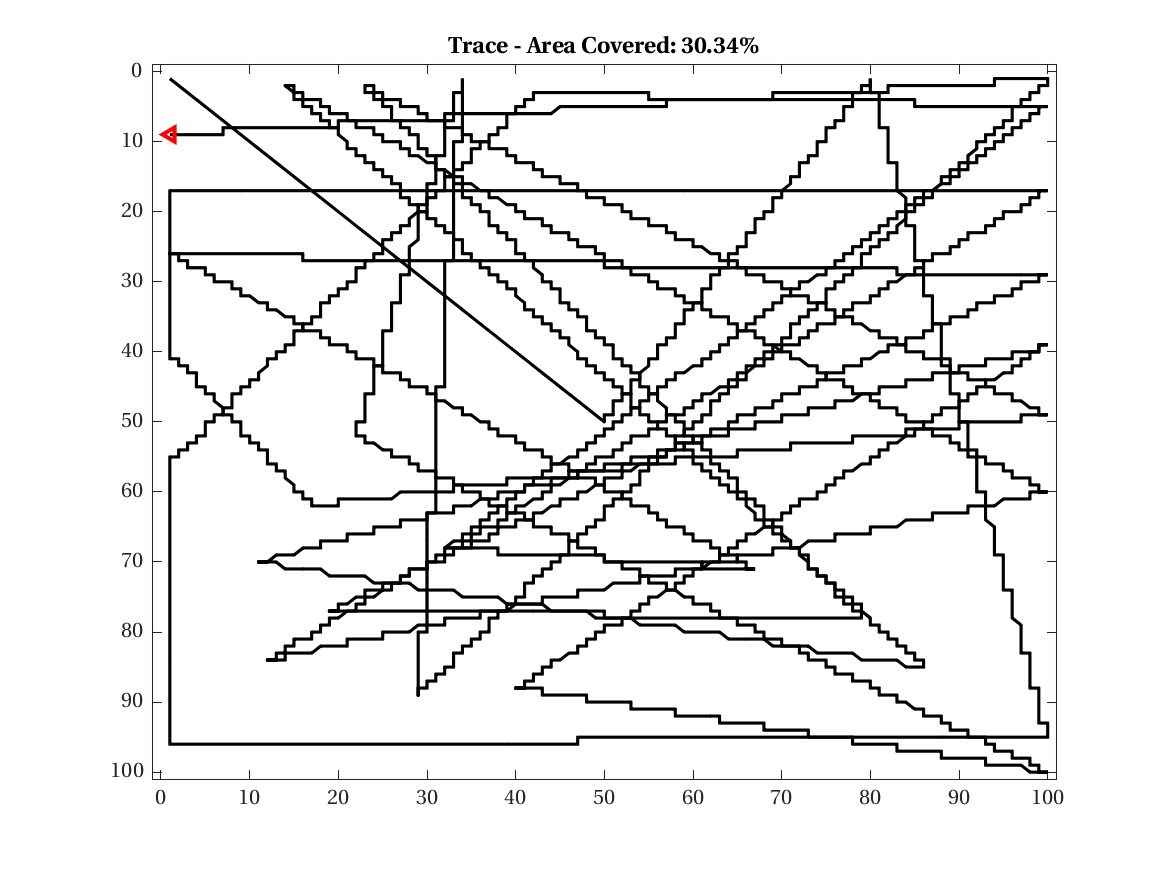
\includegraphics[width=\linewidth]{figures/path_nnhv_30p_100x100_sf_50_seed_1.png}
        \captionsetup{skip=0.20\baselineskip,size=footnotesize}
        \caption{$N$-HV}
    \end{subfigure}%
    \\
    \begin{subfigure}[t]{0.25\textwidth}
        \centering
        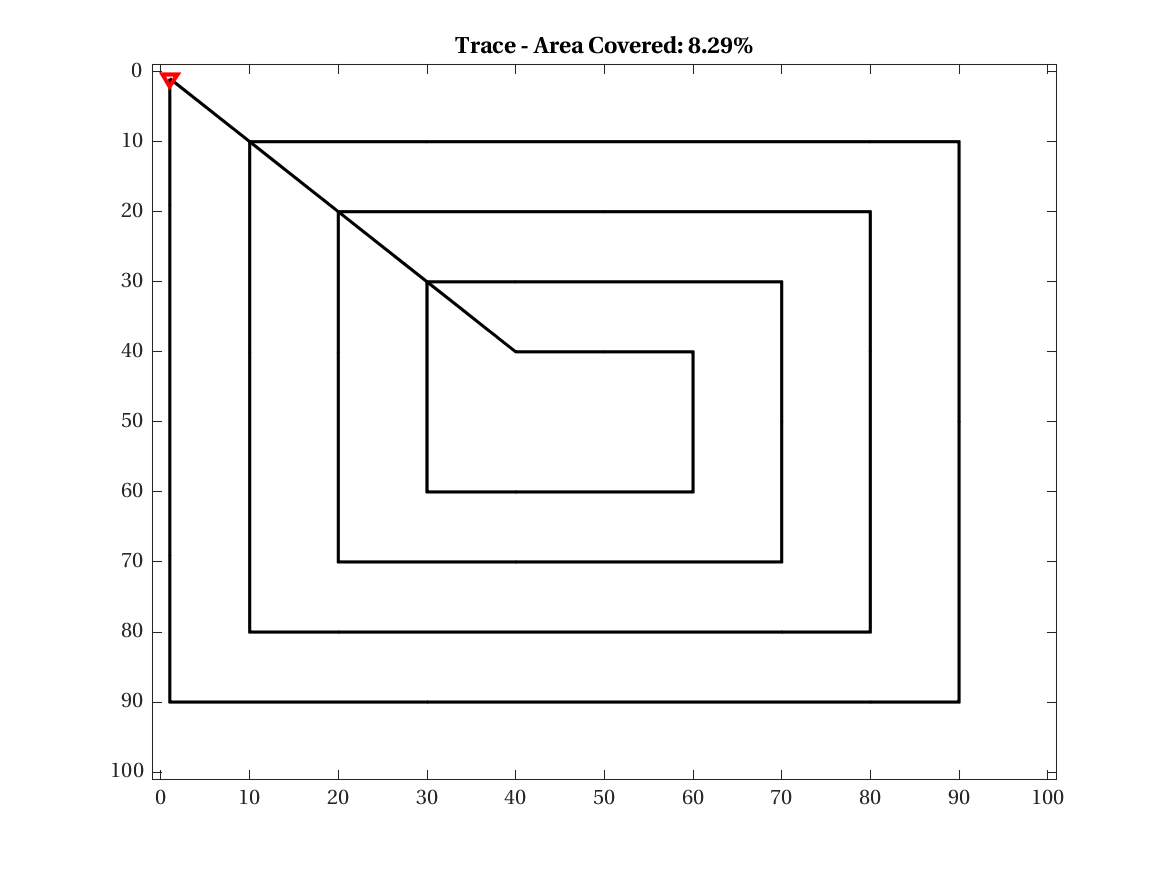
\includegraphics[width=\linewidth]{figures/path_zz_10p_100x100_sf_50_seed_1.png}
        \captionsetup{skip=0.20\baselineskip,size=footnotesize}
        \caption{$ZZ_{10}$}
    \end{subfigure}%
    \begin{subfigure}[t]{0.25\textwidth}
        \centering
        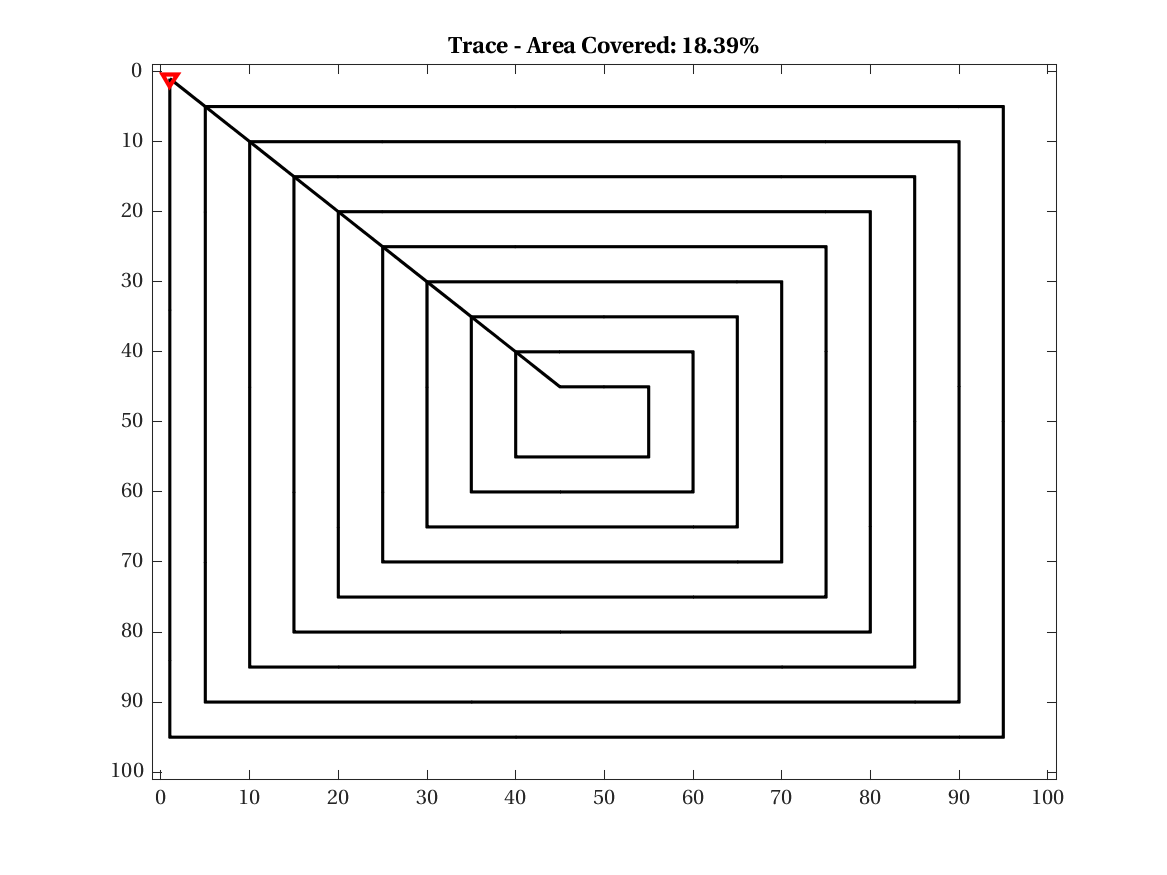
\includegraphics[width=\linewidth]{figures/path_zz_20p_100x100_sf_50_seed_1.png}
        \captionsetup{skip=0.20\baselineskip,size=footnotesize}
        \caption{$ZZ_{20}$}
    \end{subfigure}%
    \begin{subfigure}[t]{0.25\textwidth}
        \centering
        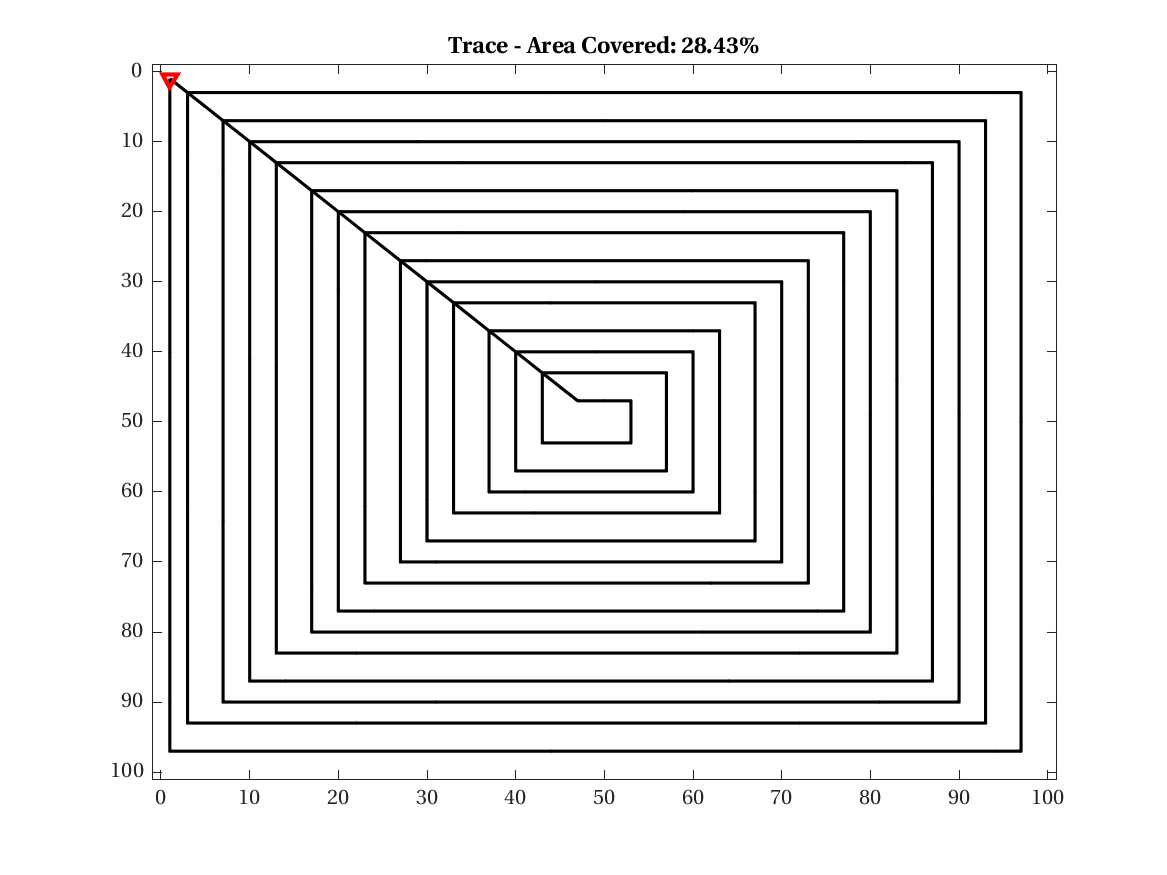
\includegraphics[width=\linewidth]{figures/path_zz_30p_100x100_sf_50_seed_1.png}
        \captionsetup{skip=0.20\baselineskip,size=footnotesize}
        \caption{$ZZ_{30}$}
    \end{subfigure}%
    \captionsetup{skip=0.20\baselineskip}
    \caption{Exploration of a field of size $100 \times 100$, $\sigma_{field} = 50$, random seed 1.}
    \label{fig:sf50}
\end{figure}

\begin{figure}[htb!]
    \centering
    \begin{subfigure}[t]{0.75\textwidth}
        \centering
        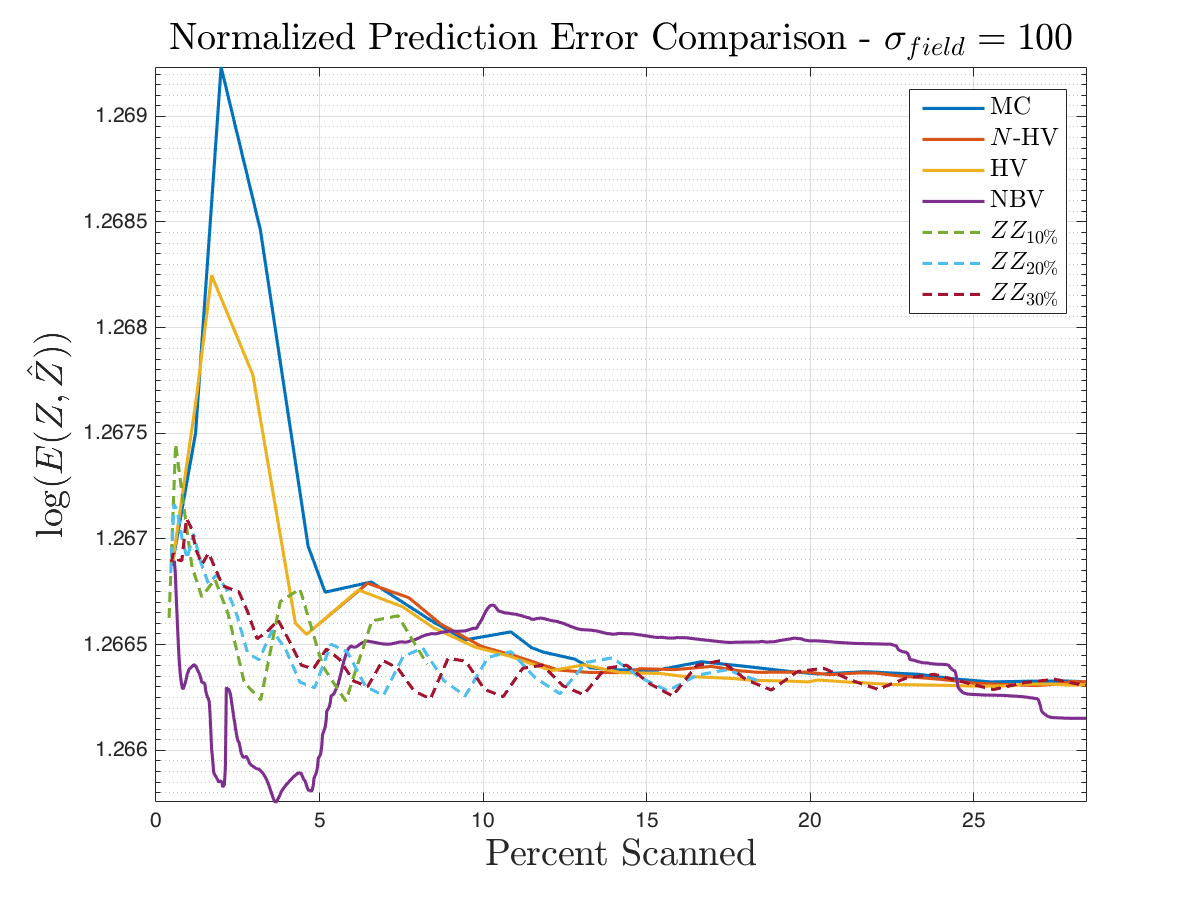
\includegraphics[width=\linewidth]{figures/normalized_errors_30p_100x100_sf_100_seed_1_app_10}
        \captionsetup{skip=0.20\baselineskip,size=footnotesize}
        \caption{Normalized prediction errors for each method.}
    \end{subfigure}%
    \\
    \begin{subfigure}[t]{0.75\textwidth}
        \centering
        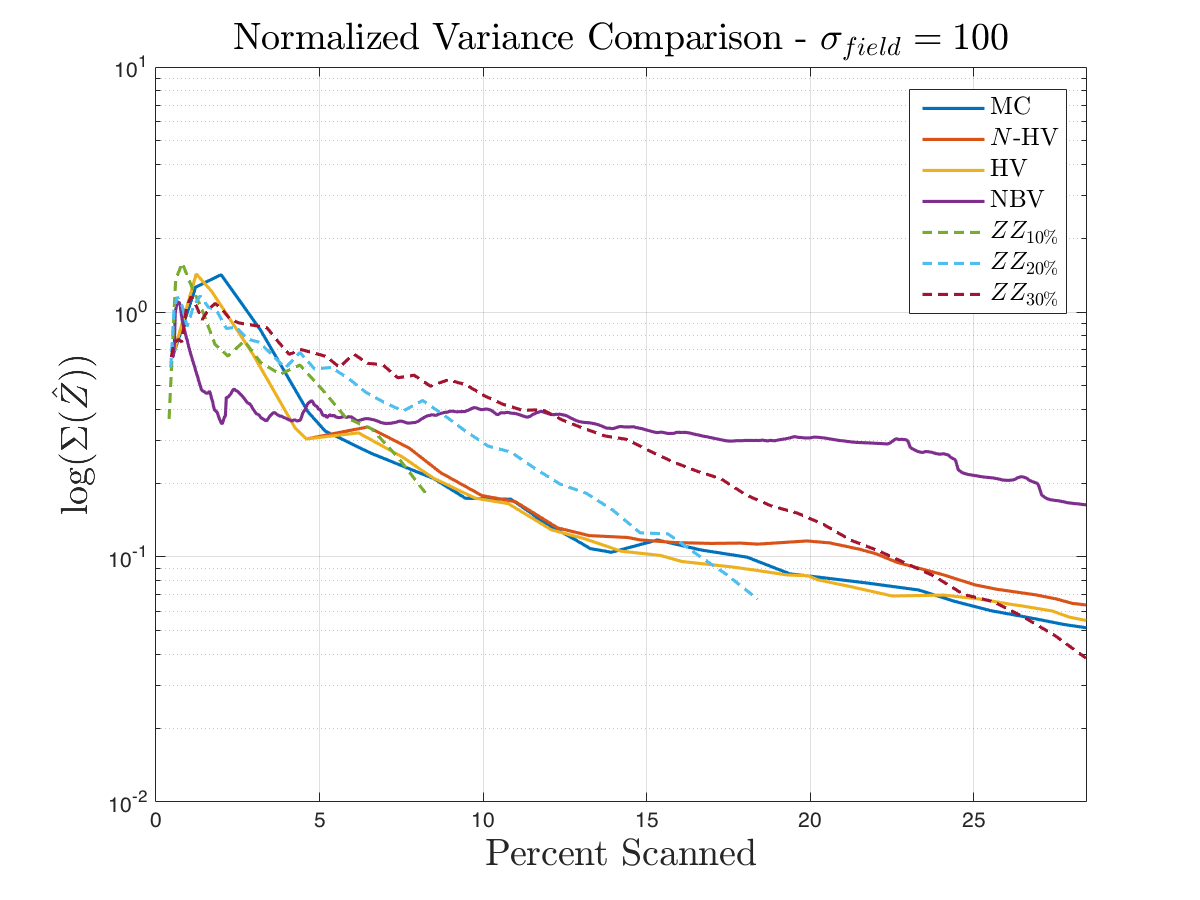
\includegraphics[width=\linewidth]{figures/normalized_variances_30p_100x100_sf_100_seed_1_app_10}
        \captionsetup{skip=0.20\baselineskip,size=footnotesize}
        \caption{Normalized prediction variances for each method.}
    \end{subfigure}%
    \captionsetup{skip=0.20\baselineskip}
    \caption{Prediction error and variances for an exploration of a field of size $100 \times 100$, $\sigma_{field} = 50$, random seed 1.}
    \label{fig:errvar50}
\end{figure}

\FloatBarrier
\clearpage

\section{Quarter Width Spatial Autocorrelation Results}
The methods will be compared on target fields generated with an autocorrelation factor, $\sigma_{field}$, that is one quarter of the field width.

\begin{figure}[htb!]
    \centering
    \begin{subfigure}[t]{0.25\textwidth}
        \centering
        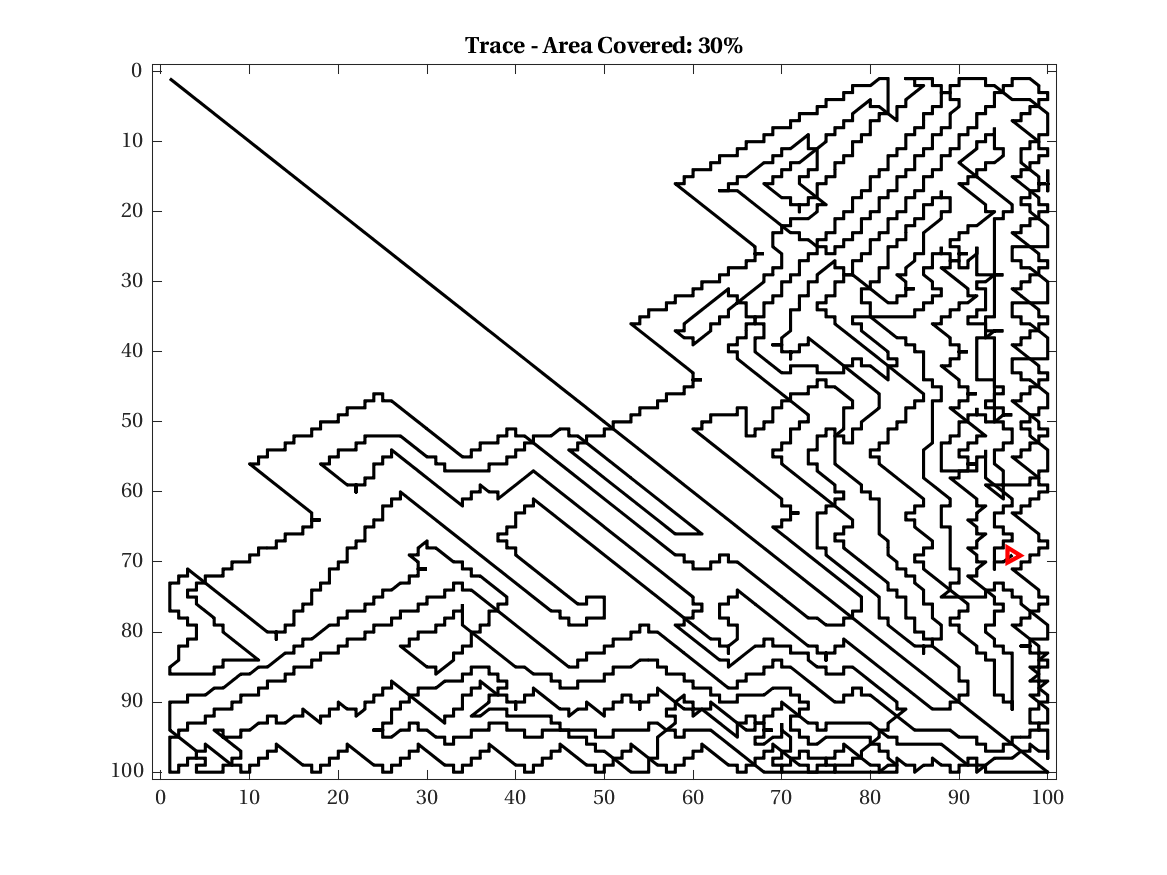
\includegraphics[width=\linewidth]{figures/path_greedy_30p_100x100_sf_25_seed_1.png}
        \captionsetup{skip=0.20\baselineskip,size=footnotesize}
        \caption{Greedy NBV}
    \end{subfigure}%
    \begin{subfigure}[t]{0.25\textwidth}
        \centering
        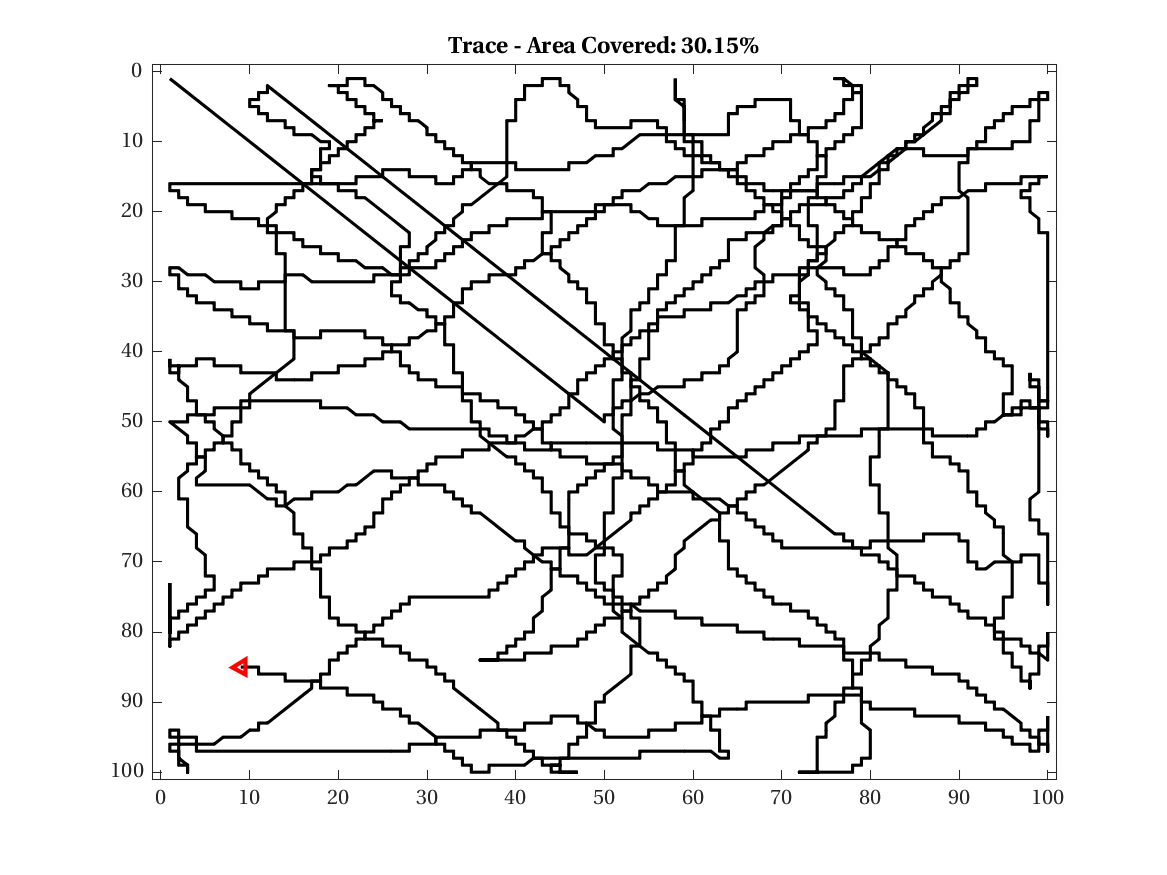
\includegraphics[width=\linewidth]{figures/path_mc_30p_100x100_sf_25_seed_1.png}
        \captionsetup{skip=0.20\baselineskip,size=footnotesize}
        \caption{MCPP}
    \end{subfigure}%
    \begin{subfigure}[t]{0.25\textwidth}
        \centering
        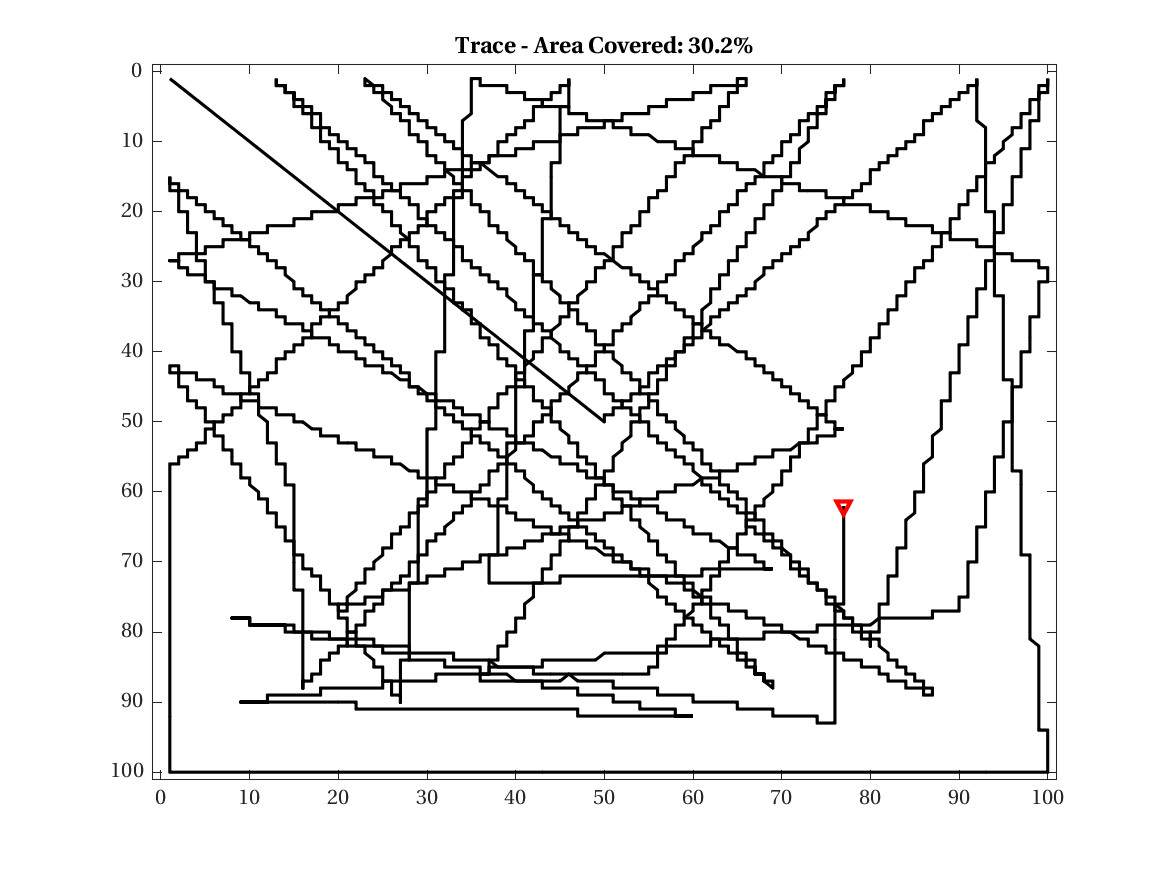
\includegraphics[width=\linewidth]{figures/path_nhv_30p_100x100_sf_25_seed_1.png}
        \captionsetup{skip=0.20\baselineskip,size=footnotesize}
        \caption{HV}
    \end{subfigure}%
    \begin{subfigure}[t]{0.25\textwidth}
        \centering
        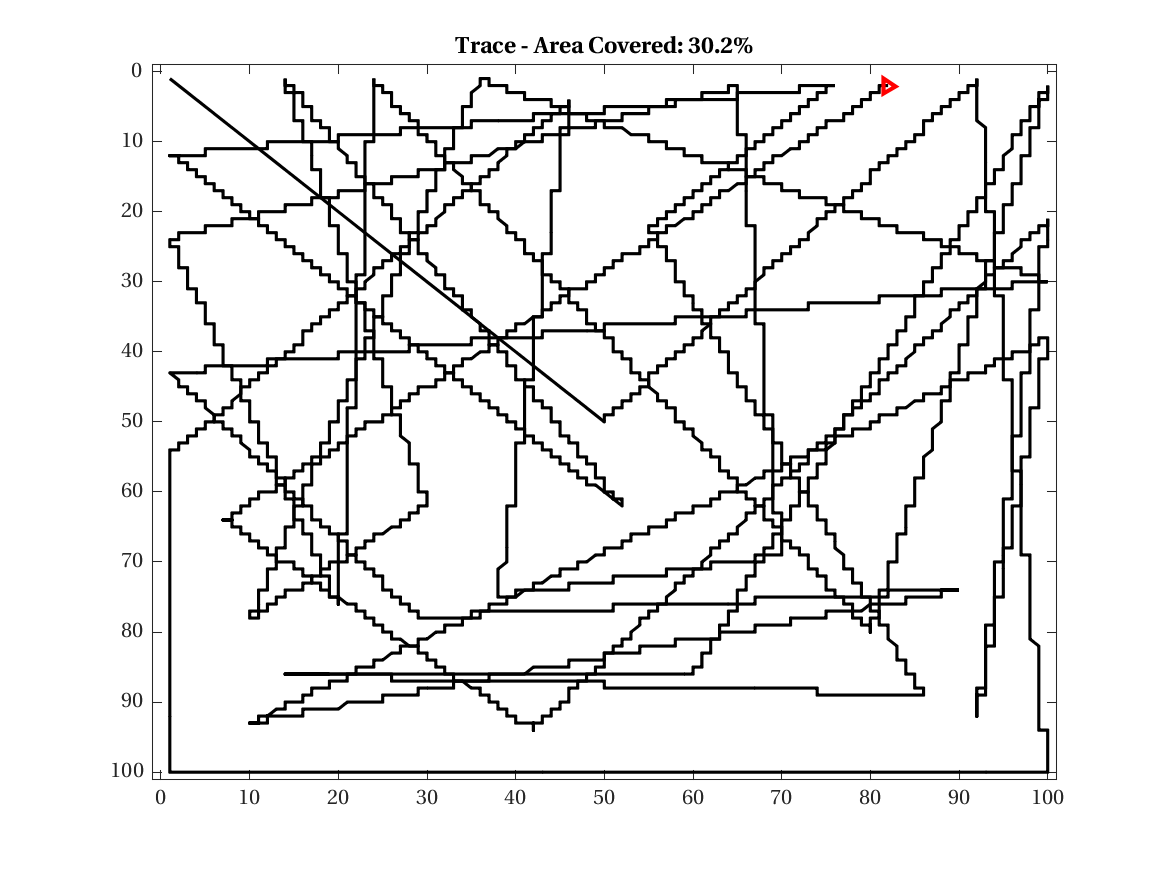
\includegraphics[width=\linewidth]{figures/path_nnhv_30p_100x100_sf_25_seed_1.png}
        \captionsetup{skip=0.20\baselineskip,size=footnotesize}
        \caption{$N$-HV}
    \end{subfigure}%
    \\
    \begin{subfigure}[t]{0.25\textwidth}
        \centering
        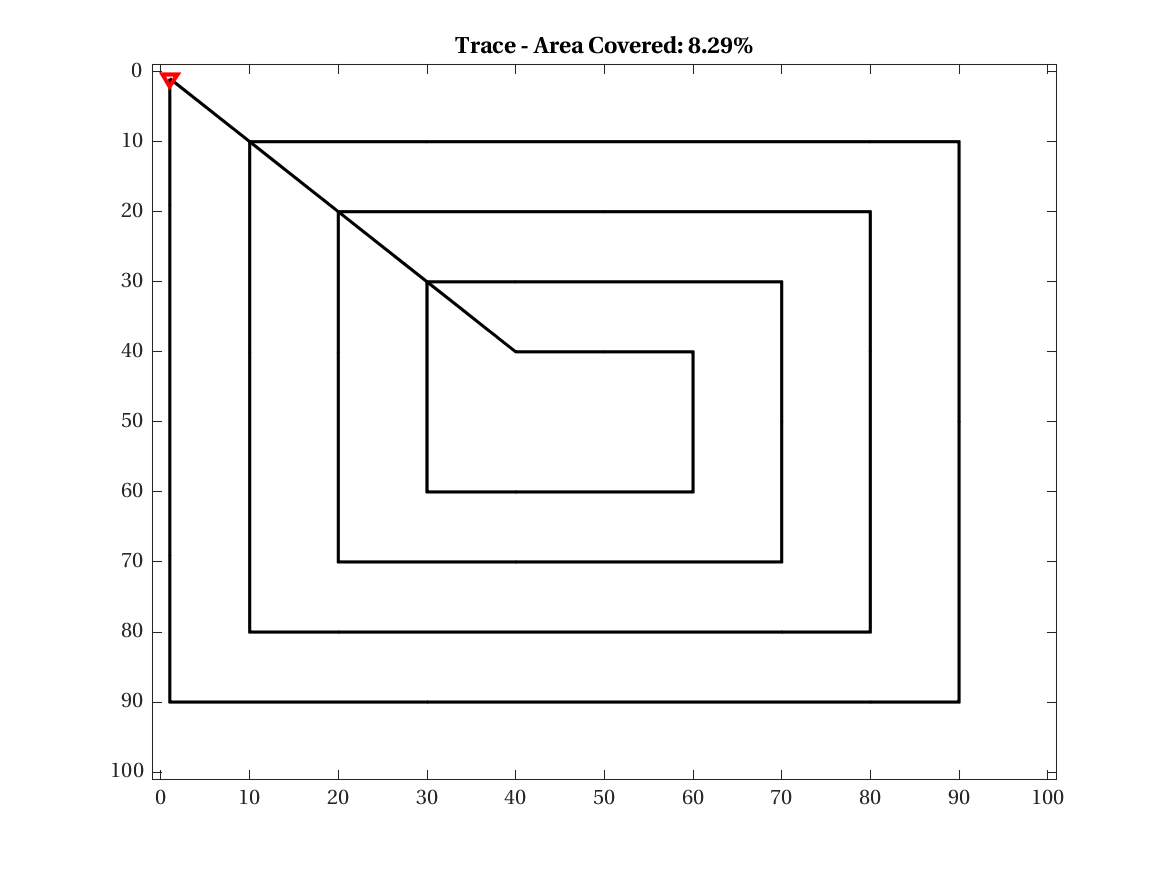
\includegraphics[width=\linewidth]{figures/path_zz_10p_100x100_sf_25_seed_1.png}
        \captionsetup{skip=0.20\baselineskip,size=footnotesize}
        \caption{$ZZ_{10}$}
    \end{subfigure}%
    \begin{subfigure}[t]{0.25\textwidth}
        \centering
        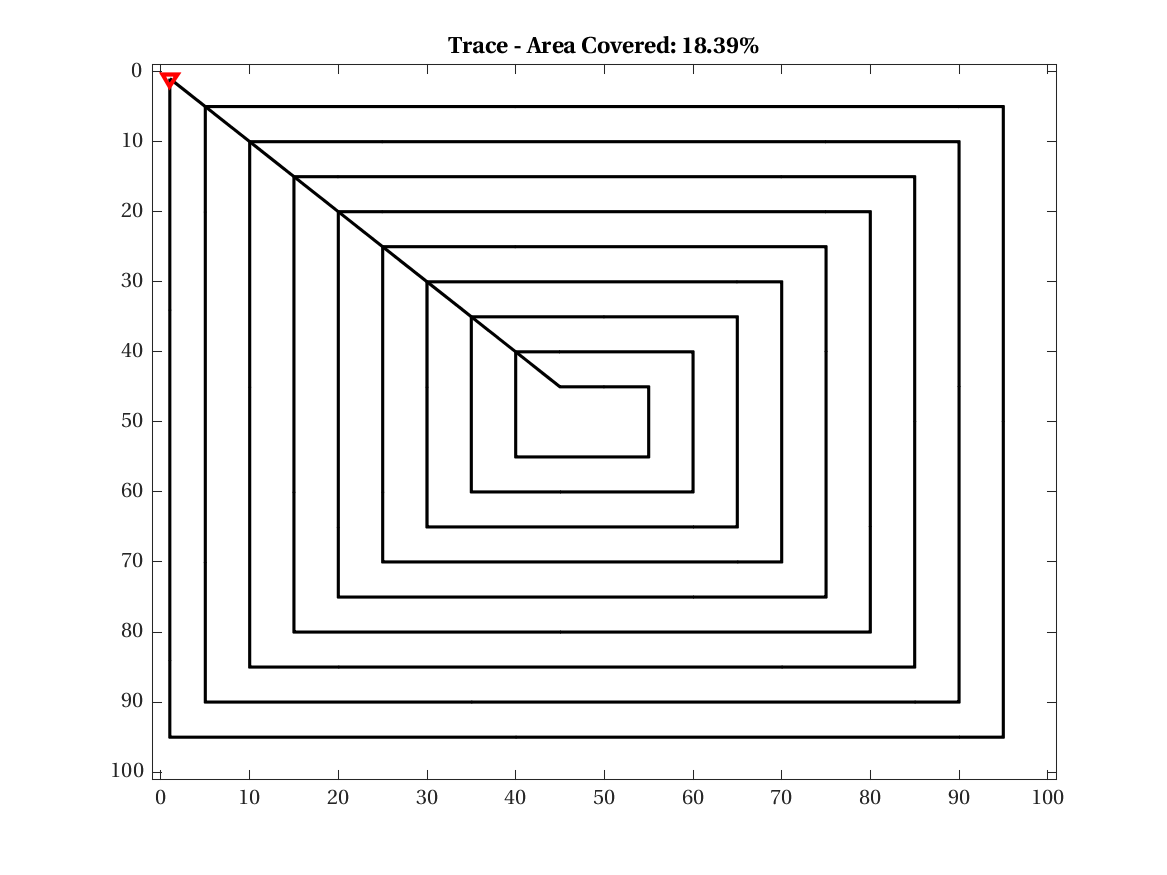
\includegraphics[width=\linewidth]{figures/path_zz_20p_100x100_sf_25_seed_1.png}
        \captionsetup{skip=0.20\baselineskip,size=footnotesize}
        \caption{$ZZ_{20}$}
    \end{subfigure}%
    \begin{subfigure}[t]{0.25\textwidth}
        \centering
        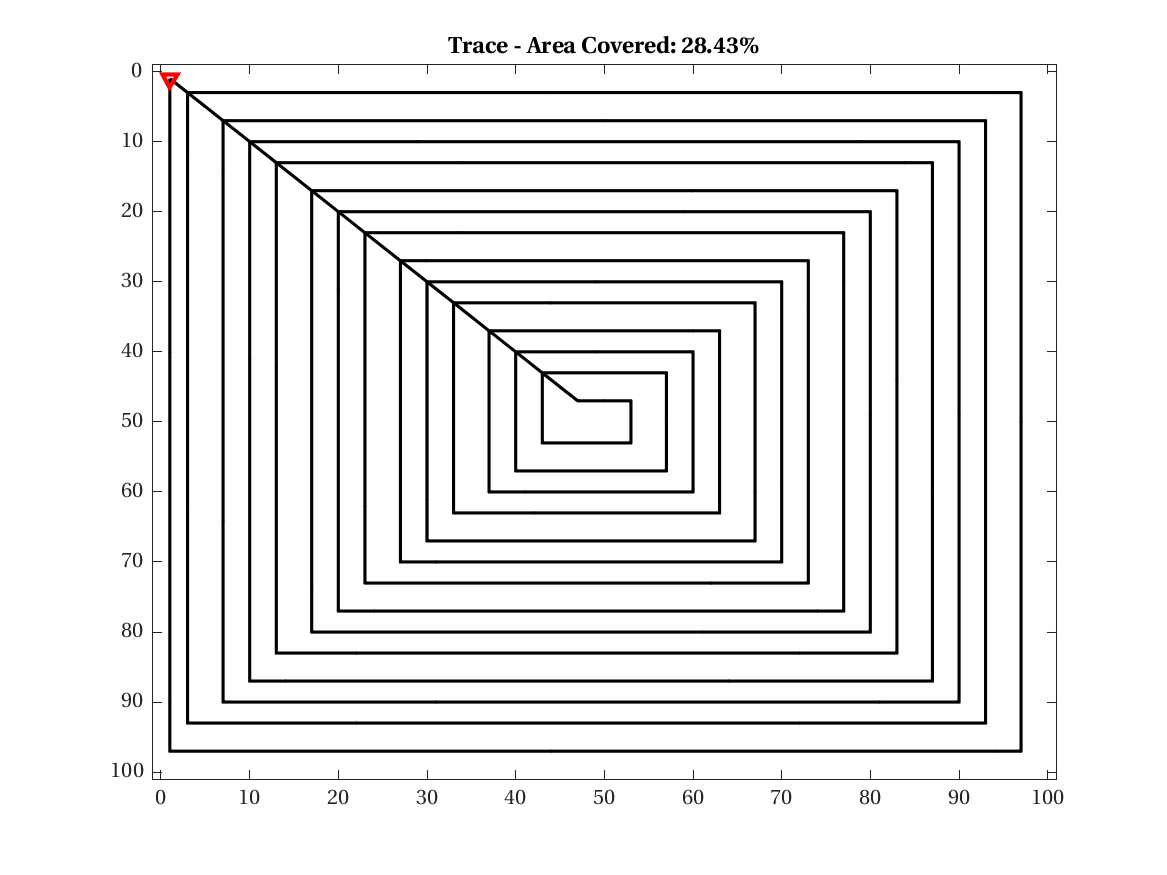
\includegraphics[width=\linewidth]{figures/path_zz_30p_100x100_sf_25_seed_1.png}
        \captionsetup{skip=0.20\baselineskip,size=footnotesize}
        \caption{$ZZ_{30}$}
    \end{subfigure}%
    \captionsetup{skip=0.20\baselineskip}
    \caption{Exploration of a field of size $100 \times 100$, $\sigma_{field} = 25$, random seed 1.}
    \label{fig:sf25}
\end{figure}

\begin{figure}[htb!]
    \centering
    \begin{subfigure}[t]{0.75\textwidth}
        \centering
        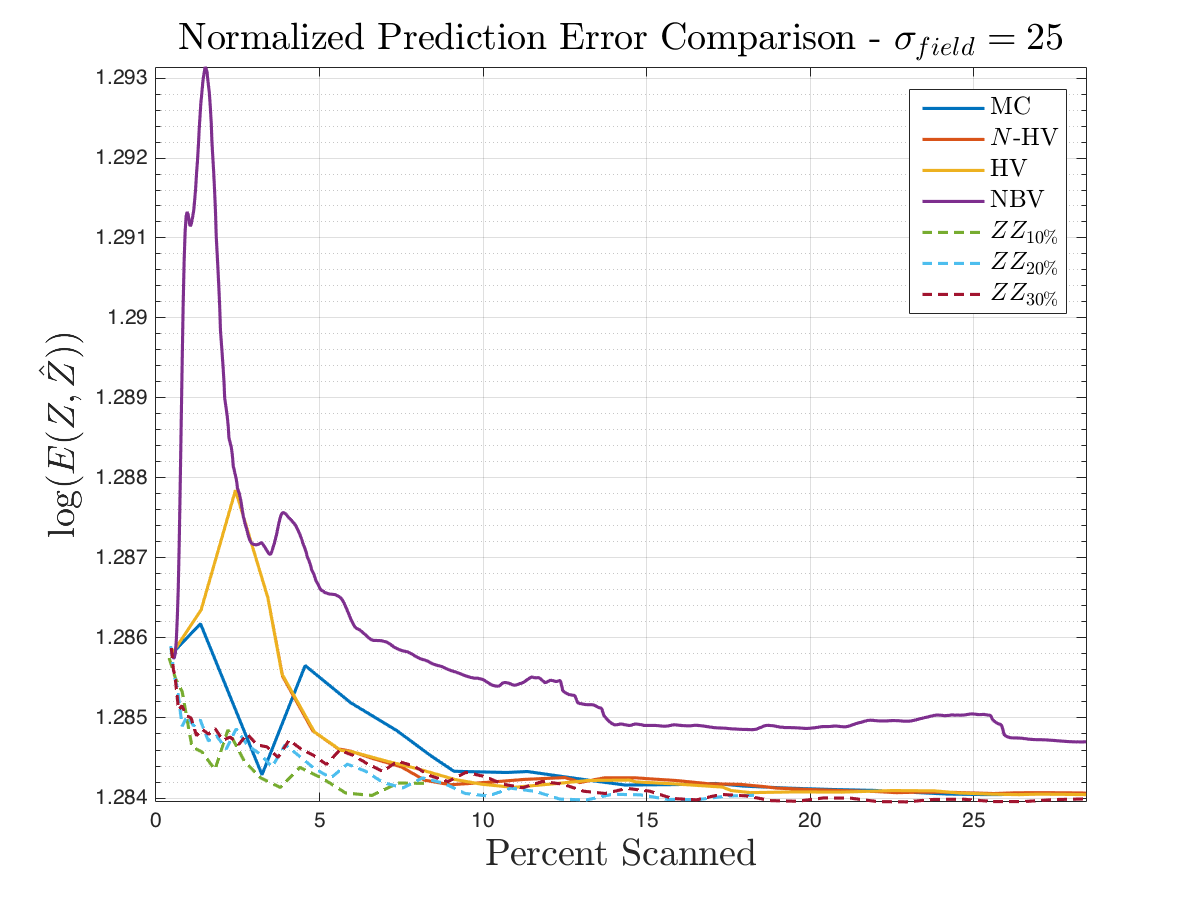
\includegraphics[width=\linewidth]{figures/normalized_errors_30p_100x100_sf_25_seed_1_app_10}
        \captionsetup{skip=0.20\baselineskip,size=footnotesize}
        \caption{Normalized prediction errors for each method.}
    \end{subfigure}%
    \\
    \begin{subfigure}[t]{0.75\textwidth}
        \centering
        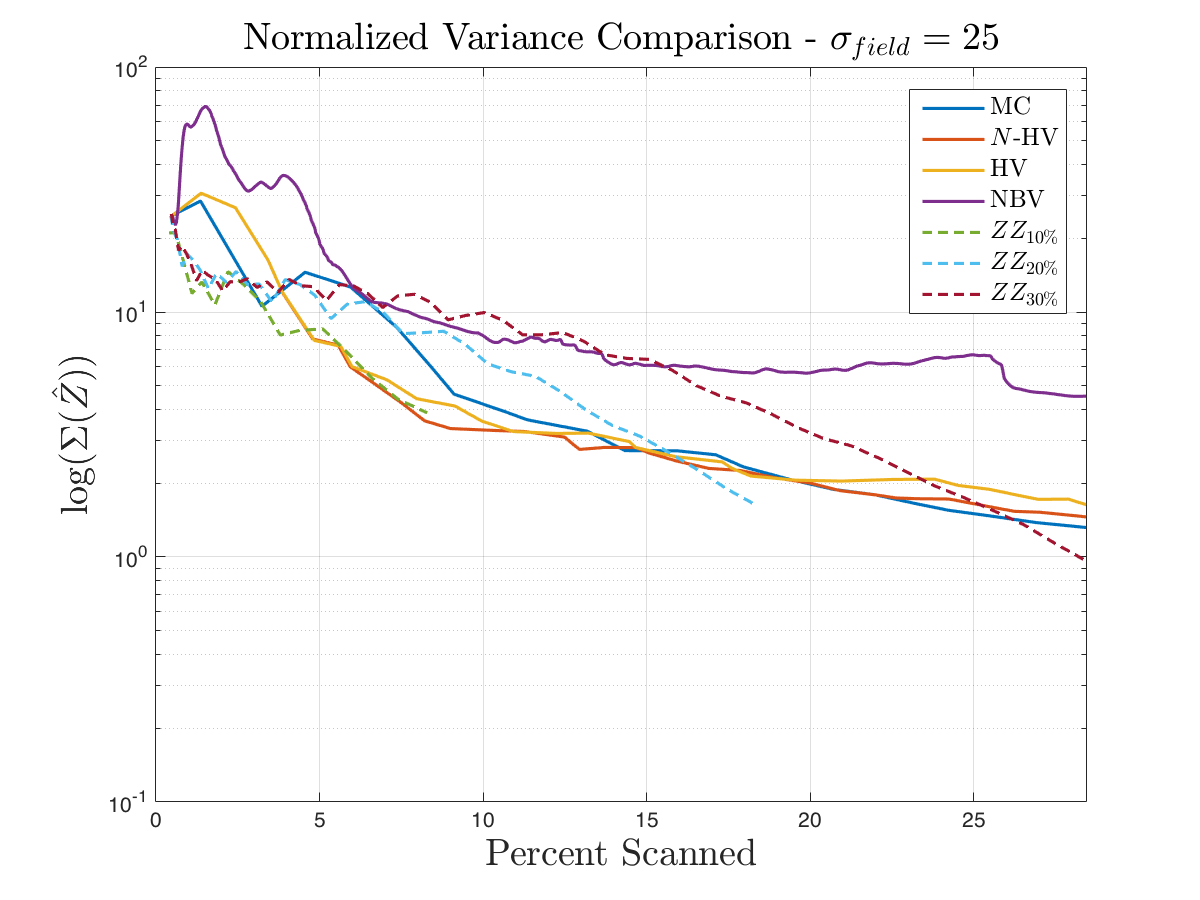
\includegraphics[width=\linewidth]{figures/normalized_variances_30p_100x100_sf_25_seed_1_app_10}
        \captionsetup{skip=0.20\baselineskip,size=footnotesize}
        \caption{Normalized prediction variances for each method.}
    \end{subfigure}%
    \captionsetup{skip=0.20\baselineskip}
    \caption{Prediction error and variances for an exploration of a field of size $100 \times 100$, $\sigma_{field} = 25$, random seed 1.}
    \label{fig:errvar25}
\end{figure}

\FloatBarrier
\clearpage

\section{Low Spatial Autocorrelation Results}
The methods will be compared on target fields generated with a low autocorrelation factor ($\sigma_{field}=1$).

\begin{figure}[htb!]
    \centering
    \begin{subfigure}[t]{0.25\textwidth}
        \centering
        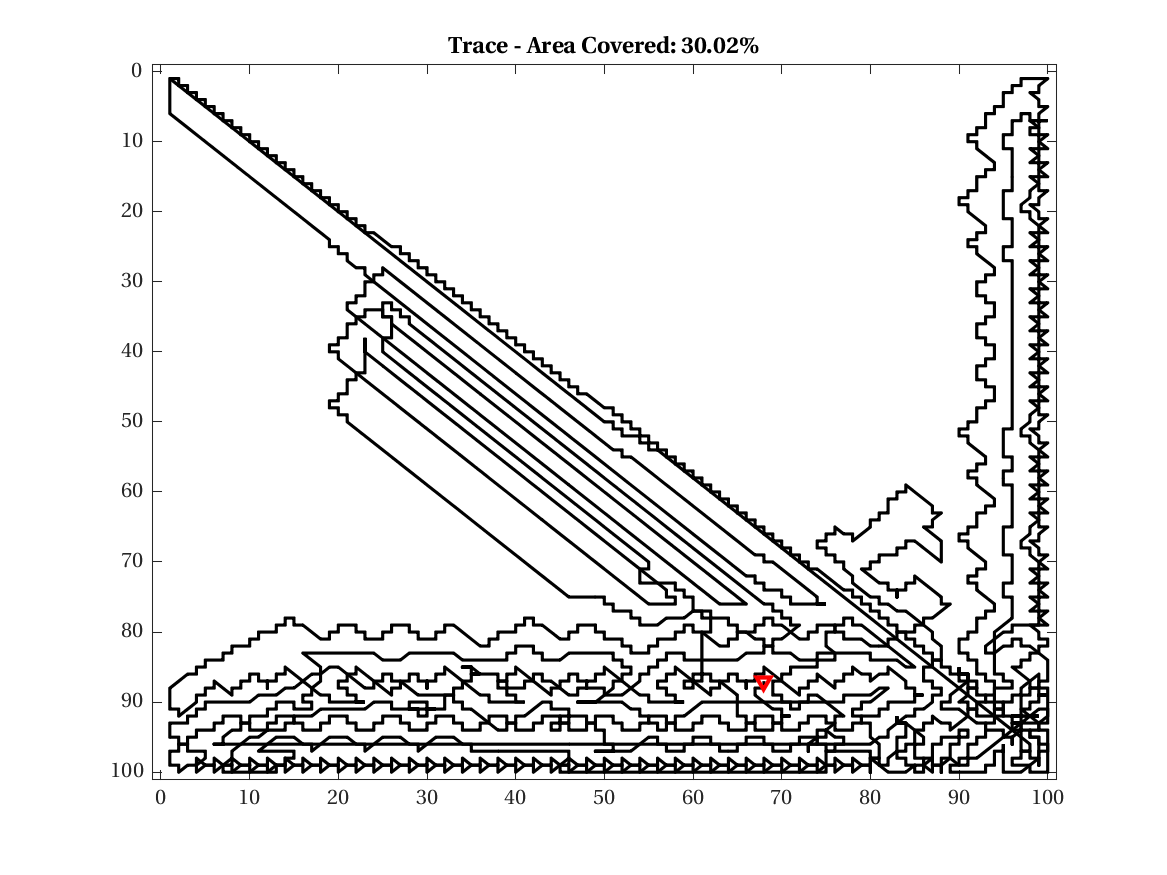
\includegraphics[width=\linewidth]{figures/path_greedy_30p_100x100_sf_1_seed_1.png}
        \captionsetup{skip=0.20\baselineskip,size=footnotesize}
        \caption{Greedy NBV}
    \end{subfigure}%
    \begin{subfigure}[t]{0.25\textwidth}
        \centering
        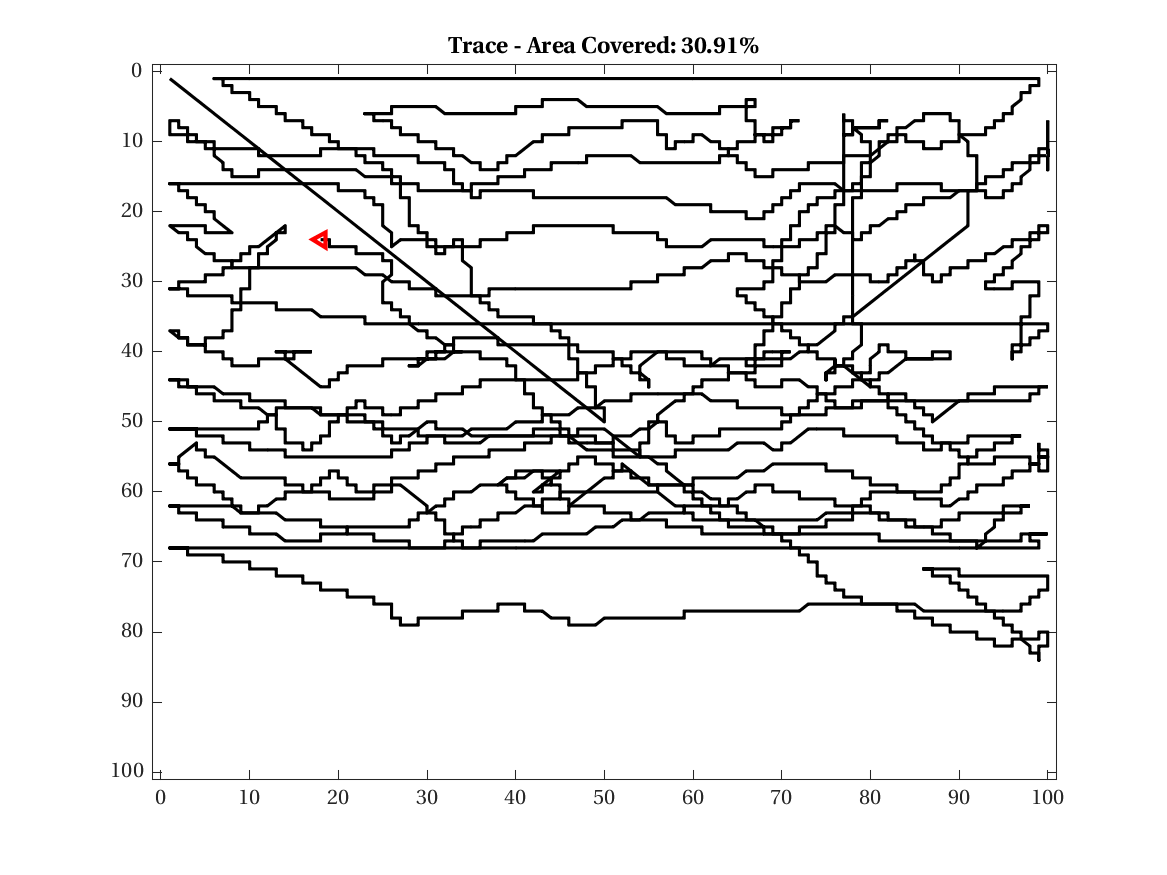
\includegraphics[width=\linewidth]{figures/path_mc_30p_100x100_sf_1_seed_1.png}
        \captionsetup{skip=0.20\baselineskip,size=footnotesize}
        \caption{MCPP}
    \end{subfigure}%
    \begin{subfigure}[t]{0.25\textwidth}
        \centering
        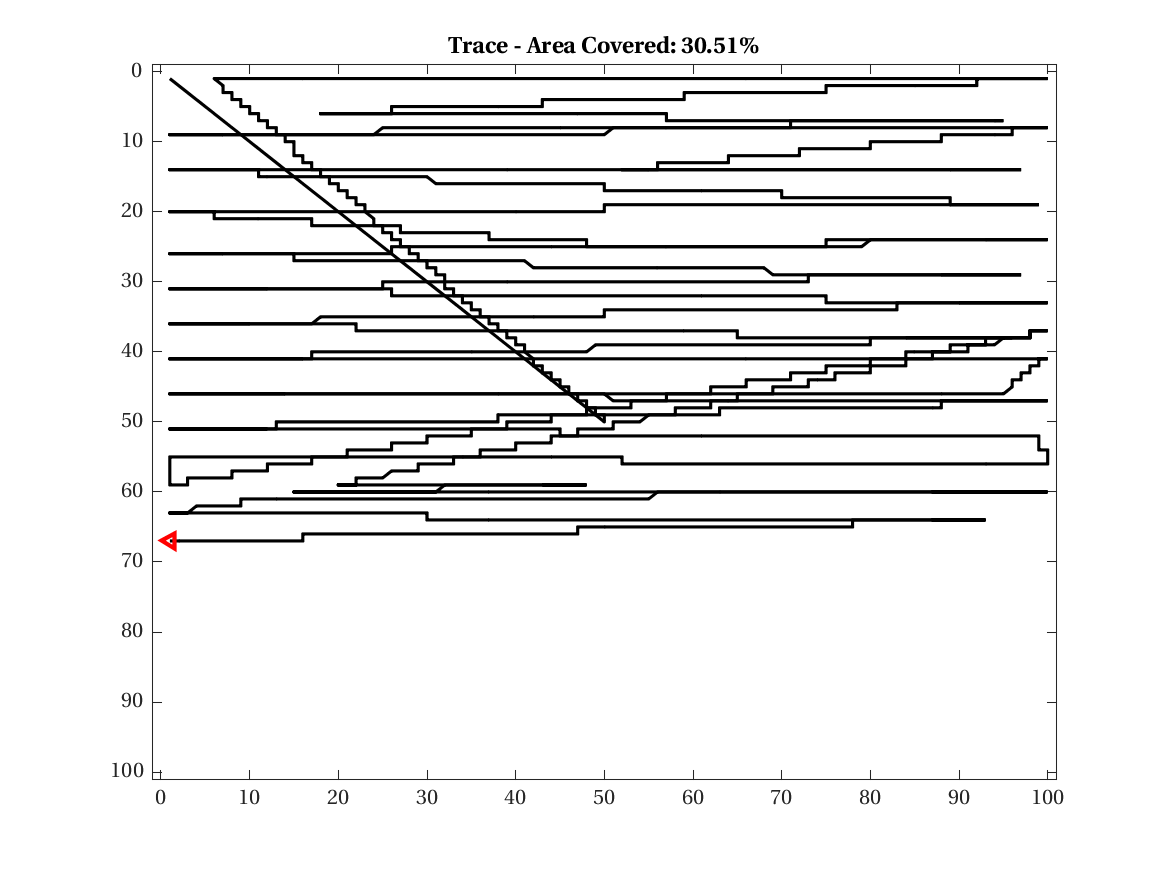
\includegraphics[width=\linewidth]{figures/path_nhv_30p_100x100_sf_1_seed_1.png}
        \captionsetup{skip=0.20\baselineskip,size=footnotesize}
        \caption{HV}
    \end{subfigure}%
    \begin{subfigure}[t]{0.25\textwidth}
        \centering
        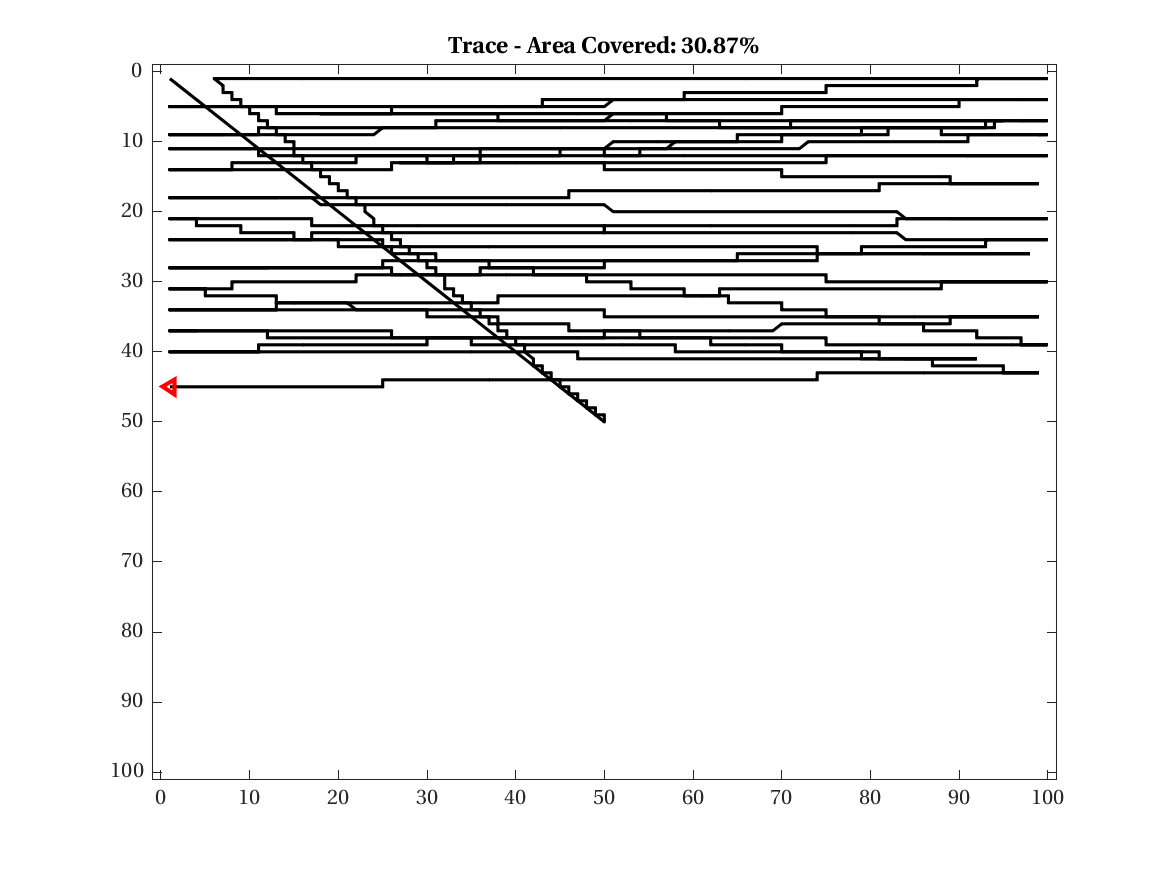
\includegraphics[width=\linewidth]{figures/path_nnhv_30p_100x100_sf_1_seed_1.png}
        \captionsetup{skip=0.20\baselineskip,size=footnotesize}
        \caption{$N$-HV}
    \end{subfigure}%
    \\
    \begin{subfigure}[t]{0.25\textwidth}
        \centering
        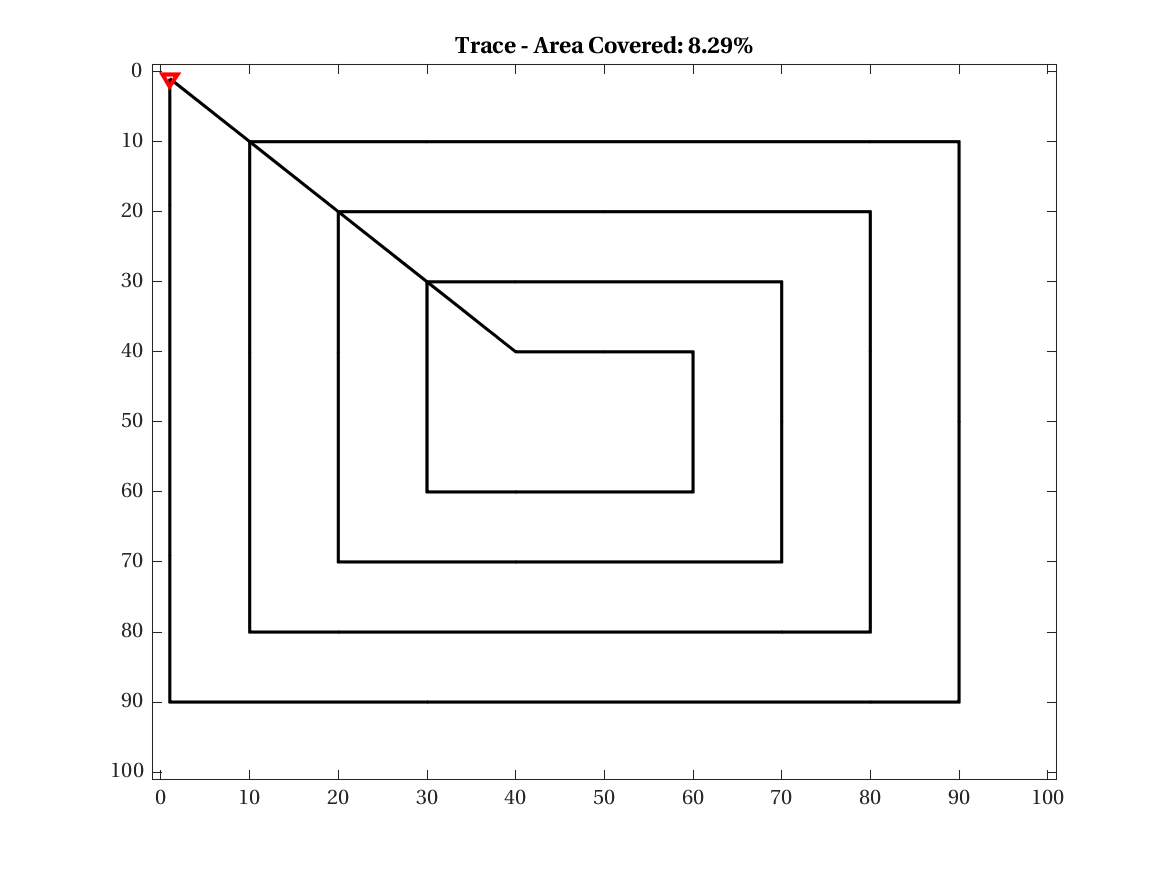
\includegraphics[width=\linewidth]{figures/path_zz_10p_100x100_sf_1_seed_1.png}
        \captionsetup{skip=0.20\baselineskip,size=footnotesize}
        \caption{$ZZ_{10}$}
    \end{subfigure}%
    \begin{subfigure}[t]{0.25\textwidth}
        \centering
        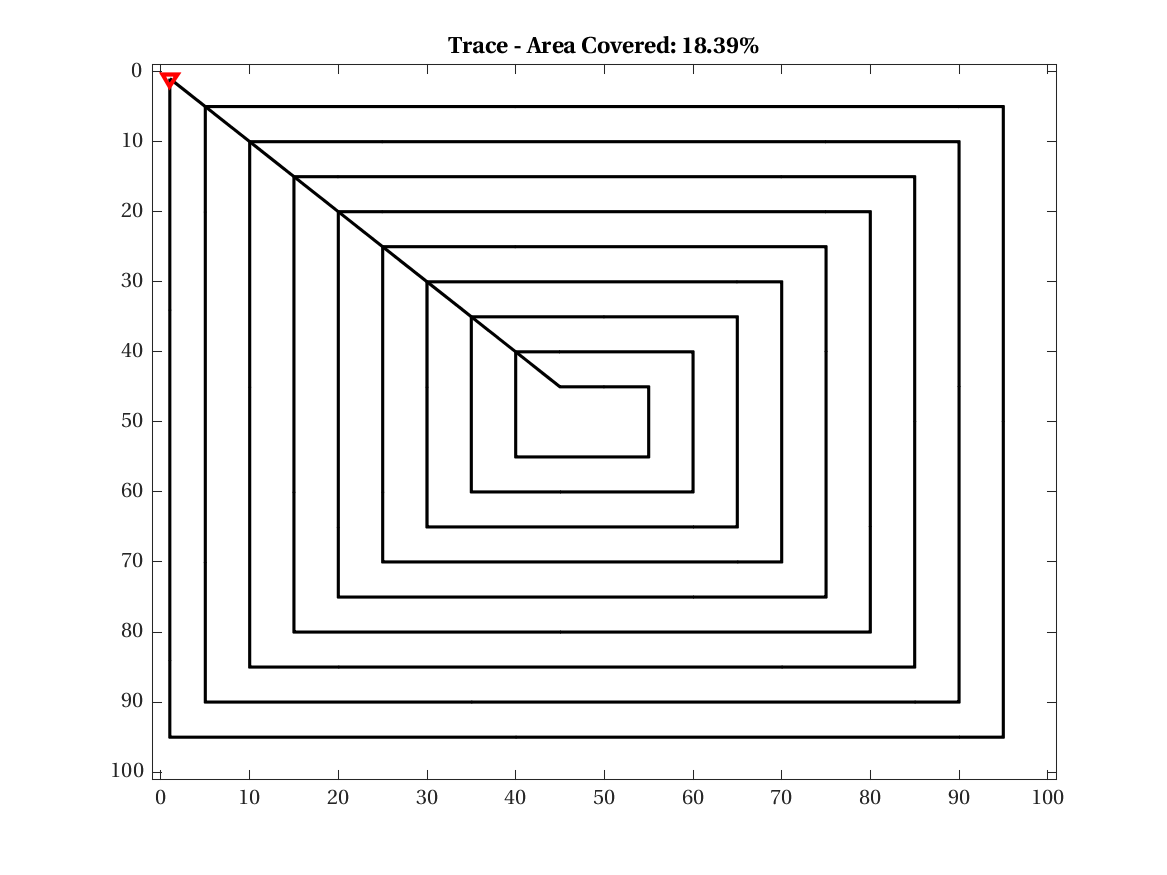
\includegraphics[width=\linewidth]{figures/path_zz_20p_100x100_sf_1_seed_1.png}
        \captionsetup{skip=0.20\baselineskip,size=footnotesize}
        \caption{$ZZ_{20}$}
    \end{subfigure}%
    \begin{subfigure}[t]{0.25\textwidth}
        \centering
        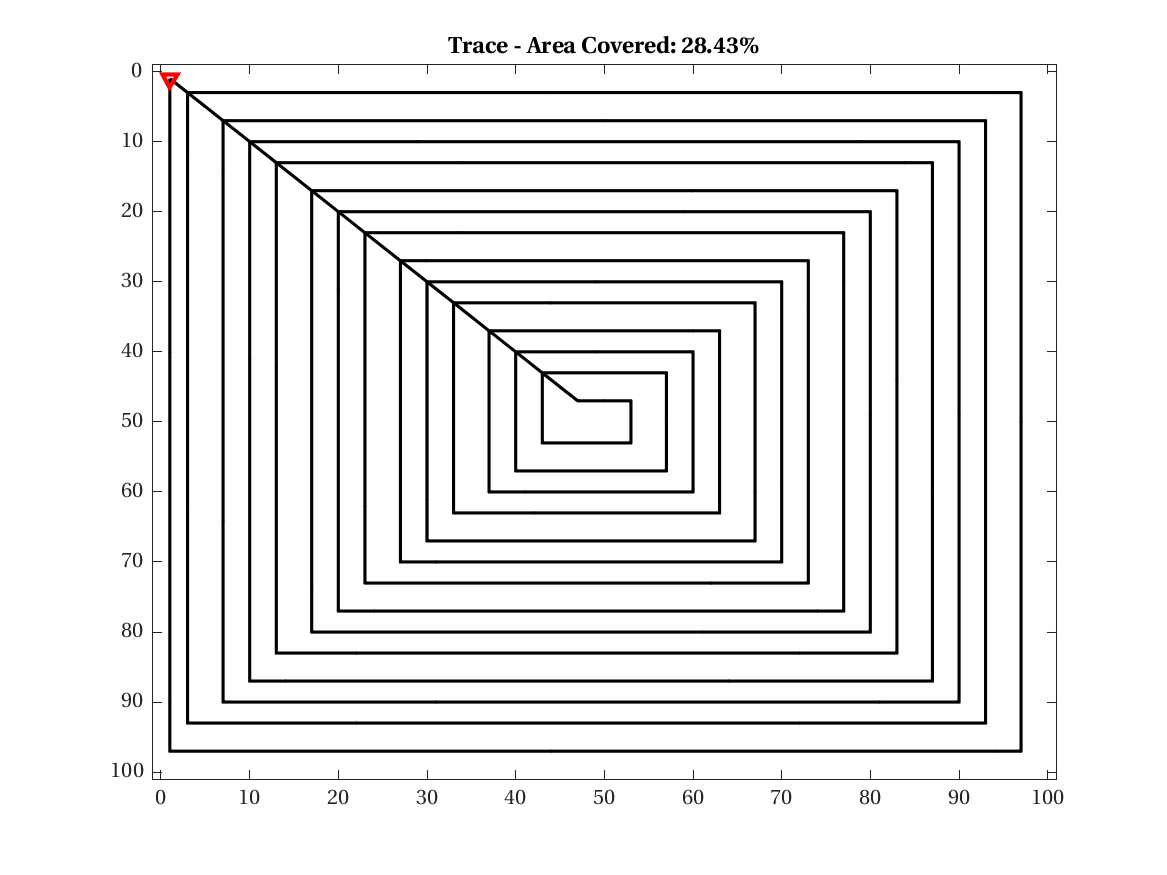
\includegraphics[width=\linewidth]{figures/path_zz_30p_100x100_sf_1_seed_1.png}
        \captionsetup{skip=0.20\baselineskip,size=footnotesize}
        \caption{$ZZ_{30}$}
    \end{subfigure}%
    \captionsetup{skip=0.20\baselineskip}
    \caption{Exploration of a field of size $100 \times 100$, $\sigma_{field} = 1$, random seed 1.}
    \label{fig:sf1}
\end{figure}

\begin{figure}[htb!]
    \centering
    \begin{subfigure}[t]{0.75\textwidth}
        \centering
        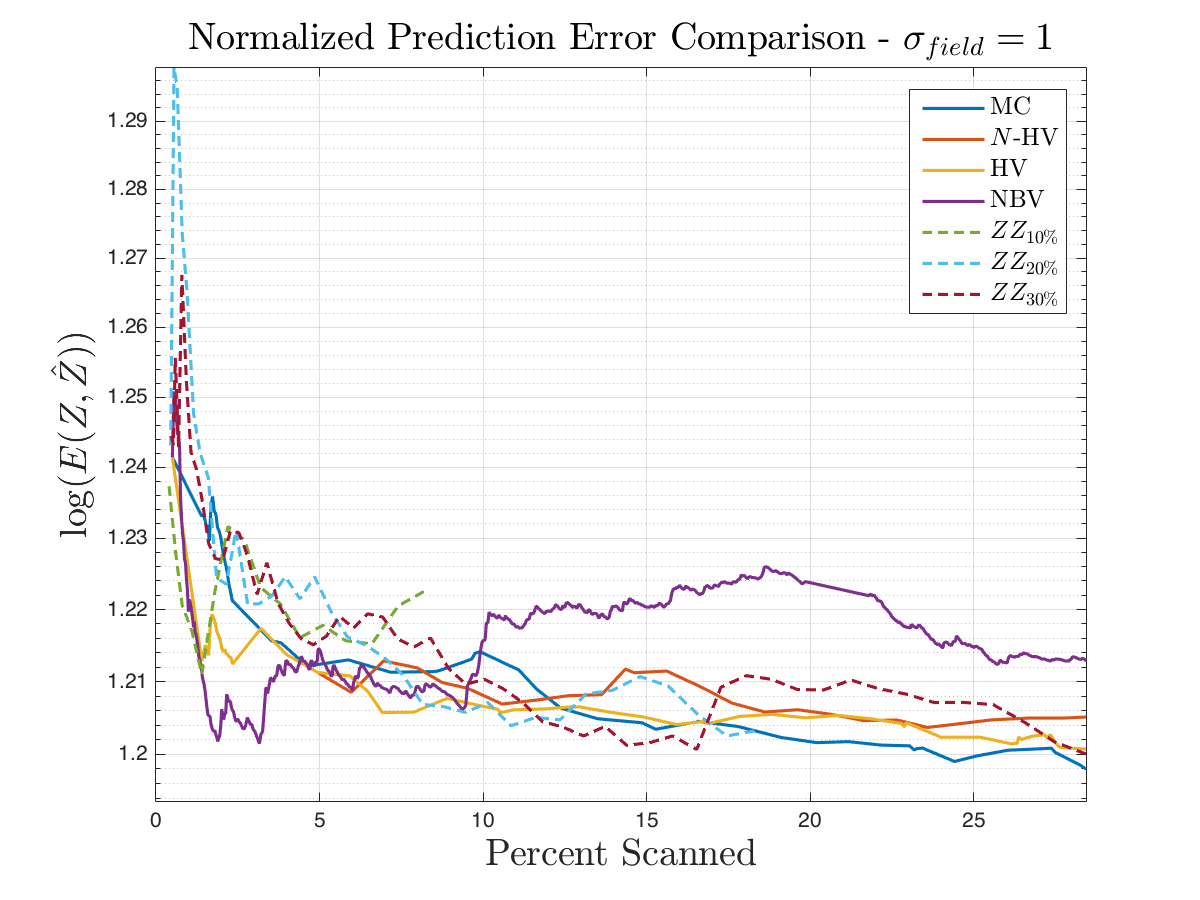
\includegraphics[width=\linewidth]{figures/normalized_errors_30p_100x100_sf_1_seed_1_app_10}
        \captionsetup{skip=0.20\baselineskip,size=footnotesize}
        \caption{Normalized prediction errors for each method.}
    \end{subfigure}%
    \\
    \begin{subfigure}[t]{0.75\textwidth}
        \centering
        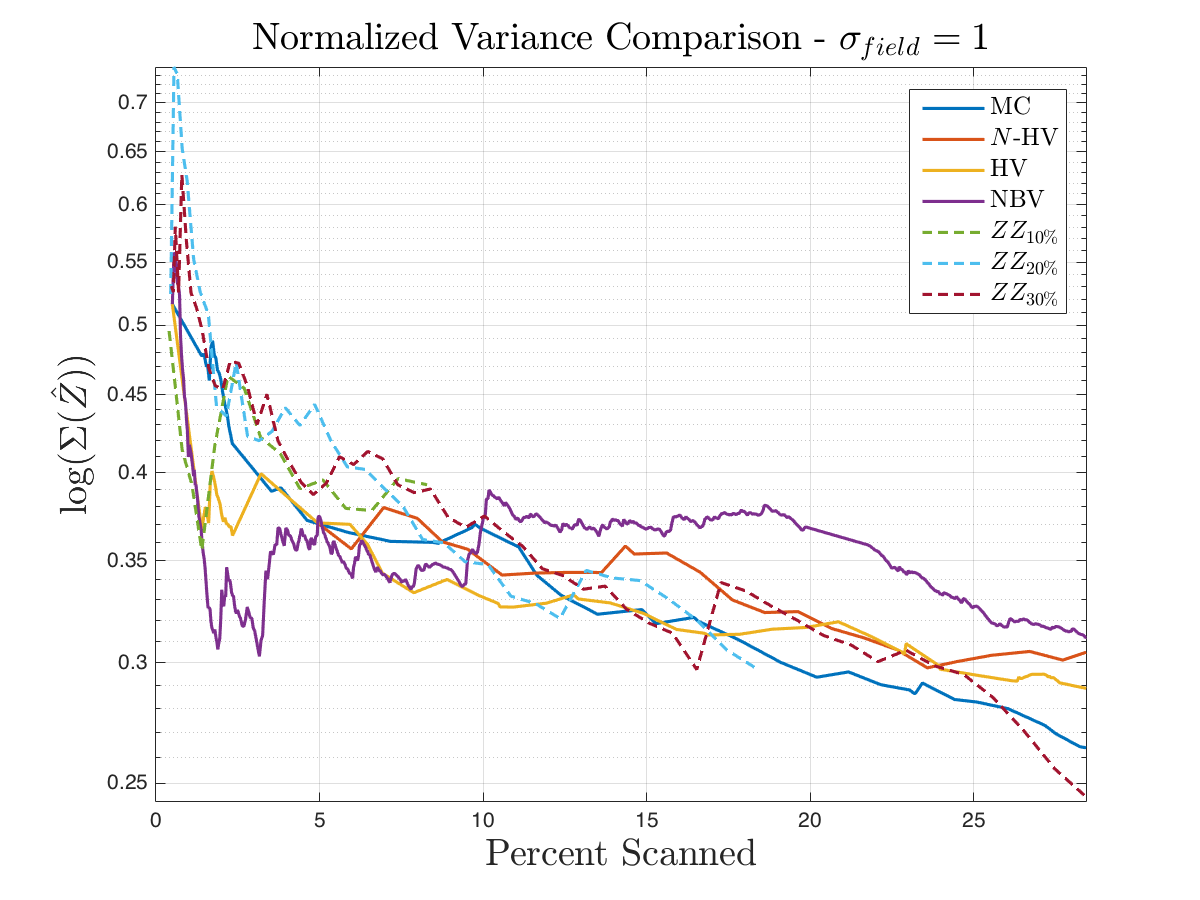
\includegraphics[width=\linewidth]{figures/normalized_variances_30p_100x100_sf_1_seed_1_app_10}
        \captionsetup{skip=0.20\baselineskip,size=footnotesize}
        \caption{Normalized prediction variances for each method.}
    \end{subfigure}%
    \captionsetup{skip=0.20\baselineskip}
    \caption{Prediction error and variances for an exploration of a field of size $100 \times 100$, $\sigma_{field} = 1$, random seed 1.}
    \label{fig:errvar1}
\end{figure}
\clearpage